\chapterimage{02_Geometrijska.jpg} % Chapter heading image

\chapter{Geometrijska optika}
V tem poglavju bomo na kratko predstavili geometrijsko optiko,
v kateri svetlobo obravnavamo kot ravne žarke. Zapisali bomo
žarkovno enačbo, vpeljali matrike ABCD za račun prehoda svetlobe
skozi optične elemente in na
primerih pokazali njihovo uporabo. Na koncu bomo opisali 
delovanje nekaterih preprostih optičnih naprav. 

\section{Fermatov teorem in optična pot}
V uvodnem zgodovinskem pregledu smo zapisali Fermatov teorem, 
ki pravi, da svetloba med dvema točkama potuje po tisti poti, 
za katero potrebuje najmanj časa. Označimo
hitrost svetlobe v snovi s $c$ in na splošno se  $c$ razlikuje
od hitrosti svetlobe v praznem prostoru $c_0$. Razmerje med
hitrostjo svetlobe v praznem prostoru in njeno hitrostjo
v snovi opisuje lomni količnik $n$. Velja:
\boxeq{eq:c}{
c = \frac{c_0}{n}.
}
Hitrost svetlobe v praznem prostoru je
po definiciji enaka $c_0 = 299\,\,792\,\,458~\si{m/s}$, 
lomni količnik pa je odvisen od snovi in frekvence svetlobe: za vidno svetlobo
je v vodi približno $1,3$, v steklih okoli $1,4$--$1,9$ in v diamantu $2,4$.

Naj svetloba potuje po snovi z lomnim količnikom $n$. Celotno pot, ki 
jo svetloba opravi od začetne do končne točke, razdelimo na kratke intervale 
poti $ds$. Za del poti $ds$ potrebuje svetloba čas $dt$, ki ga zapišemo kot:
\begin{equation}
 dt = \frac{ds}{c} = \frac{ds}{c_0/n} = \frac{nds}{c_0}.
\label{eq:02_02}
\end{equation}
Fermatov teorem pravi, da svetloba potuje po poti, za katero velja:
\beq
\int_1^2 dt = \int_1^2 \frac{nds}{c_0} = \mathrm{min}.
\label{eq:02_03}
\eeq
Če je lomni količnik konstanten, svetloba potuje naravnost in 
ne spreminja smeri. Na splošno pa se lomni količnik spreminja s 
krajem, zato teorem prepišemo v:
\boxeq{eq:02_04}{
S = \int_1^2 n(\mathbf{r})ds = \mathrm{min}.
}
Celotni integral $S$ imenujemo optična pot, ki se od geometrijske poti razlikuje v tem,
da upošteva tudi lomni količnik snovi. 
Zapisani izraz imenujemo princip najmanjše optične poti oziroma najmanjše optične akcije. 
Problem je podoben principu najmanjše akcije v klasični mehaniki, zato včasih govorimo  
tudi o Langrangeevi oziroma Hamiltonovi optiki.
\begin{remark}
Princip najkrajše optične poti lahko formalno izpeljemo z 
obravnavo valovnih front in žarkov v valovni optiki, če naredimo limito $\lambda \to 0$.
Tako lahko izhajajoč iz Maxwellovih enačb pokažemo pravilnost Fermatovega teorema.
\end{remark}

\begin{example}
{\bf Izpeljava lomnega zakona iz Fermatovega teorema.}
Naj svetlobni žarek vpada na ravno mejo dveh snovi. Levo od meje je snov 
z lomnim količnikom $n_1$, desno pa snov z lomnim količnikom $n_2$. Naj svetloba
potuje od točke 1, ki jo izberemo na oddaljenosti $z_1$ levo 
od meje, do točke 2 na oddaljenosti $z_2$ desno od meje. Vzdolžna razdalja med obema
točkama naj bo $x$ (slika~\ref{fig:02_FerLom}). 
\begin{figure}[ht]
\centering
\def\svgwidth{100truemm} 
\input{slike/02_FerLom.pdf_tex}
\caption{K izračunu loma na meji dveh snovi}
\label{fig:02_FerLom}
\end{figure}

Naša naloga je poiskati pot žarka svetlobe od točke 1 do točke 2 ob pogoju, 
da je skupna optična pot najkrajša.
Celotno optično pot zapišemo kot:
\begin{equation}
S = n_1 s_1 + n_2 s_2 = n_1 \sqrt{x_1^2+z_1^2}\, +\, n_2 \sqrt{x_2^2+z_2^2}.
\label{eq:02_05}
\end{equation}
Izrazimo parameter $x_2$ z lego iskane točke $x_1$: 
\begin{equation}
S = n_1 \sqrt{x_1^2+z_1^2}\, +\, n_2 \sqrt{(x-x_1)^2+z_2^2}.
\label{eq:02_06}
\end{equation}
Najkrajšo optično pot izračunamo tako, da poiščemo vrednost $x_1$, 
pri kateri je odvod optične poti po $x_1$ enak nič. Zapišemo:
\begin{equation}
\frac{dS}{dx_1} = \frac{2 n_1 x_1}{2 \sqrt{x_1^2+z_1^2}}+
\frac{-2n_2 (x-x_1)}{2 \sqrt{(x-x_1)^2+z_2^2}} = 0.
\label{eq:02_07}
\end{equation}
Vpeljemo vpadni kot $\alpha$ glede na normalo na mejo snovi (slika~\ref{fig:02_FerLom}):
\begin{equation}
\sin \alpha = \frac{x_1}{\sqrt{x_1^2+z_1^2}}.
\label{eq:02_08}
\end{equation}
Lomni kot $\beta$ naj bo kot med smerjo žarka v drugi snovi in normalo na mejo snovi: 
\begin{equation}
\sin \beta = \frac{x_2}{\sqrt{x_2^2+z_2^2}} = \frac{(x-x_1)}{\sqrt{(x-x_1)^2+z_2^2}}.
\label{eq:02_09}
\end{equation}
Vstavimo enačbi~(\ref{eq:02_08}) in (\ref{eq:02_09}) v enačbo~(\ref{eq:02_07})
in dobimo lomni zakon v znani obliki:
\boxeq{eq:lomnizakon}{
n_1 \sin \alpha = n_2 \sin \beta.
}
Na podoben način izpeljemo tudi odbojni zakon, tako da izračunamo 
najkrajšo optično pot med točkama 1 in 3. Dobimo:
\boxeq{eq:odbojnizakon}{
\tilde{\alpha} = \alpha.
}
\end{example}

\section{Žarkovna enačba}
\label{chap:zarkovna}
Poglejmo, kako izračunamo najkrajšo optično pot v primeru, ko 
meja med dvema snovema ni ostra, ampak se lomni količnik zvezno spreminja. 
Naj bo lomni količnik v splošnem funkcija kraja: $n = n(\mathbf{r}) = n(x,y,z)$.
Numerično se naloge lotimo tako, da snov razdelimo
na kratke odseke in na mejah med njimi uporabimo lomni ali odbojni zakon.
Analitično problem rešujemo z uporabo Euler-Lagrangeeve enačbe za minimum
funkcionala optične poti $S$:
\begin{equation}
 S = \int_1^2 n(x,y,z) ds  = \int_1^2 n(x,y,z)\,|\mathbf{v}|\,dt  = 
 \int_1^2 n(x,y,z) \sqrt{\dot{x}^2+ \dot{y}^2+\dot{z}^2} dt,
 \label{eq:02_10}
\end{equation}
pri čemer pika označuje odvod posamezne koordinate po času. Integrand
enačbe predstavlja Langrangian $L$, ki je funkcija treh koordinat in njihovih
odvodov.
\begin{equation}
L(x, y, z, \dot{x}, \dot{y}, \dot{z}) = n(x,y,z) \sqrt{\dot{x}^2+ \dot{y}^2+\dot{z}^2}.
\label{eq:02_11}
\end{equation}
Lagrangian vstavimo v Euler-Lagrangeevo enačbo\footnote{~Glej npr. P. Prelovšek, {\it Klasična
mehanika}, skripta, 2013.} in za koordinato $x$ dobimo:
\begin{equation}
 \frac{d}{dt}\left(\frac{\partial L}{\partial \dot{x}}\right) - 
 \frac{\partial L}{\partial x} = 0.
 \label{eq:02_12}
\end{equation}
Vstavimo Langrangian (enačba~\ref{eq:02_11}) 
v enačbo~(\ref{eq:02_12}) in dobimo:
\begin{equation}
\frac{d}{dt}\left(n \frac{\dot{x}}{\sqrt{\dot{x}^2+ \dot{y}^2+\dot{z}^2}} \right)
 = \frac{\partial n}{\partial x}\sqrt{\dot{x}^2+ \dot{y}^2+\dot{z}^2}.
  \label{eq:02_13}
\end{equation}
Pomnožimo enačbo z $dt/ds$:
\begin{equation}
\frac{d}{dt}\left(n \frac{\dot{x}}{\sqrt{\dot{x}^2+ \dot{y}^2+\dot{z}^2}} \right)
\frac{dt}{ds}
 = \frac{\partial n}{\partial x}\frac{\sqrt{\dot{x}^2+ \dot{y}^2+\dot{z}^2}\,dt}{ds}.
  \label{eq:02_14}
\end{equation}
Na desni strani enačbe uporabimo zvezo:
\begin{equation}
 \sqrt{\dot{x}^2+ \dot{y}^2+\dot{z}^2} dt = ds,
 \label{eq:02_15}
\end{equation}
na levi strani pa verižno pravilo odvajanja, po katerem lahko pokrajšamo $dt$. Dobimo:
\begin{equation}
 \frac{d}{ds} \left( n \frac{dx}{dt\sqrt{\dot{x}^2+ \dot{y}^2+\dot{z}^2}} \right)=
 \frac{\partial n}{\partial x}.
 \label{eq:02_16}
\end{equation}
Enačbo~(\ref{eq:02_15}) uporabimo še enkrat v oklepaju na levi strani. Sledi:
\begin{equation}
 \frac{d}{ds} \left( n\, \frac{dx}{ds} \right)=
 \frac{\partial n}{\partial x}.
  \label{eq:02_17}
\end{equation}
Podobni enačbi zapišemo še za koordinati $y$ in $z$, nato vse tri enačbe
združimo v enotno žarkovno enačbo:
\boxeq{eq:zarkovnaenacba}{
\nabla n = \frac{d}{ds} \left( n \frac{d\mathbf{r}}{ds}\right)\!.
}
Rešitev žarkovne enačbe poda trajektorijo optičnega žarka v parametrični 
obliki $\mathbf{r}(s)$. Z uporabo zveze $ds = dz (1+(dx/dz)^2+(dy/dz)^2)^{1/2}$
lahko enačbo prevedemo na sistem diferencialnih enačb za $x(z)$ in $y(z)$. Reševanje
tega sistema enačb je na splošno zelo zapleteno.

\begin{example}
{\bf Žarkovna enačba v homogeni snovi.} Naj svetloba potuje po snovi,
v kateri je lomni količnik konstanten. Potem je $\nabla n = 0$ in 
\begin{equation}
0 = \frac{d}{ds}\left( n \frac{d\mathbf{r}}{ds} \right) = 
n \frac{d^2 \mathbf{r}}{ds^2}.
 \label{eq:02_18}
\end{equation}
Rešitev te enačbe je ravni žarek:
\begin{equation}
 \mathbf{r} = \mathbf{a}_0+\mathbf{a}_1\,s,
  \label{eq:02_19}
\end{equation}
pri čemer vektor $\mathbf{a}_0$ opisuje lego začetne točke, 
vektor $\mathbf{a}_1$ pa ima smer od začetne do končne točke.
\end{example}

\subsection*{Obosni približek žarkovne enačbe}
V optiki pogosto privzamemo, da smer širjenja svetlobe le malo 
odstopa od neke dane smeri. Naj bo to smer $z$, ki jo imenujemo
optična os sistema. Zaradi enostavnosti se omejimo na ravninski primer, 
tako da trajektorijo žarka opazujemo v ravnini $xz$ 
(slika~\ref{fig:02_FerOs}). Lomni količnik naj bo funkcija $n= n(x)$.
\begin{figure}[ht]
\centering
\def\svgwidth{90truemm} 
\input{slike/02_FerOs.pdf_tex}
\caption{K zapisu žarkovne enačbe v obosnem približku}
\label{fig:02_FerOs}
\end{figure}

Predpostavko, da se žarek širi pretežno v smeri $z$ in od te smeri 
le malo odstopa, matematično zapišemo s pogojem:
\begin{equation}
 \frac{dx}{dz}\ll 1.
  \label{eq:02_20}
\end{equation}
Iz tega sledi, da za naklon žarka $\vartheta$, ki ga na danem mestu izračunamo kot:
\begin{equation}
\vartheta = \frac{dx}{dz}
 \label{eq:02_21}
\end{equation}
velja $\sin \vartheta \approx \tan \vartheta \approx \vartheta \ll 1$.
Upoštevajoč enačbo~(\ref{eq:02_20}) zapišemo:
\begin{equation}
ds = \sqrt{dx^2+dz^2} = \sqrt{1+\left(\frac{dx}{dz}\right)^2}\,\,dz \approx dz.
\label{eq:02_22}
\end{equation}
Predpostavki, da se žarek širi približno vzdolž osi $z$, pravimo
obosni ali paraksialni približek. V nadaljevanju se ga bomo še velikokrat 
posluževali. Žarkovno enačbo (enačba~\ref{eq:zarkovnaenacba}) v obosnem približku
zapišemo kot:
\begin{equation}
 \frac{dn}{dx} = \frac{d}{dz}\left(n(x)\,\frac{dx}{dz}\right) = n(x)\,\frac{d^2x}{dz^2}
  \label{eq:02_23}
\end{equation}
oziroma
\boxeq{eq:02_24}{
\frac{d^2x}{dz^2} = \frac{1}{n(x)} \frac{dn}{dx}.
}

\begin{example}
{\bf Žarkovna enačba v snovi s paraboličnim profilom
lomnega količnika.} Izračunajmo trajektorijo žarka svetlobe v 
obosnem približku v snovi, v kateri se lomni količnik parabolično 
spreminja z oddaljenostjo od osi $z$.  Odvisnost lomnega količnika 
od oddaljenosti $x$ od osi $z$ zapišemo kot:
\begin{equation}
 n(x) = n_0 \left(1-\frac{\alpha^2\,x^2}{2}\right)\!,
 \label{eq:02_25}
\end{equation}
pri čemer je $\alpha x$ majhen.
Vstavimo izraz za lomni količnik (enačba~\ref{eq:02_25}) v obosni približek
žarkovne enačbe (enačba~\ref{eq:02_24}) in dobimo:
\begin{equation}
 \frac{d^2x}{dz^2}= \frac{1}{n(x)}\frac{dn}{dx} = 
 \frac{-n_0 \alpha^2x}{n_0 \left(1-\alpha^2\,x^2/2\right)} 
 \approx -\frac{n_0\alpha^2x}{n_0} = -\alpha^2x.
 \label{eq:02_26}
\end{equation}
Enačbo~(\ref{eq:02_26}) preprosto rešimo in dobimo splošno 
obliko trajektorije:
\begin{equation}
 x(z) = A \cos (\alpha z) + B \sin (\alpha z).
  \label{eq:02_27}
\end{equation}
Naj bo v izhodišču pri $z=0$ žarek na oddaljenosti $x_0$ 
in naj se širi pod kotom $\vartheta_0$. 
Z upoštevanjem začetnih pogojev dobimo rešitev:
\begin{equation}
x (z) = x_0 \cos(\alpha z) + \frac{\vartheta_0}{\alpha} \sin (\alpha z).
 \label{eq:02_28}
\end{equation}
Rešitve obosnega približka žarkovne enačbe v snovi s paraboličnim profilom 
so torej oscilatorne funkcije s periodo $2\pi/\alpha$ (glej sliko~\ref{fig:02_FerPar}).
\begin{figure}[ht]
\centering
\def\svgwidth{100truemm} 
\input{slike/02_FerPar.pdf_tex}
\caption{Rešitev žarkovne enačbe v snovi s paraboličnim profilom lomnega
količnika je periodična. Narisanih
je šest žarkov, pri katerih je $x_0=0$, razlikujejo pa se v $\vartheta_0$.}
\label{fig:02_FerPar}
\end{figure}

\begin{figure}[ht]
\centering
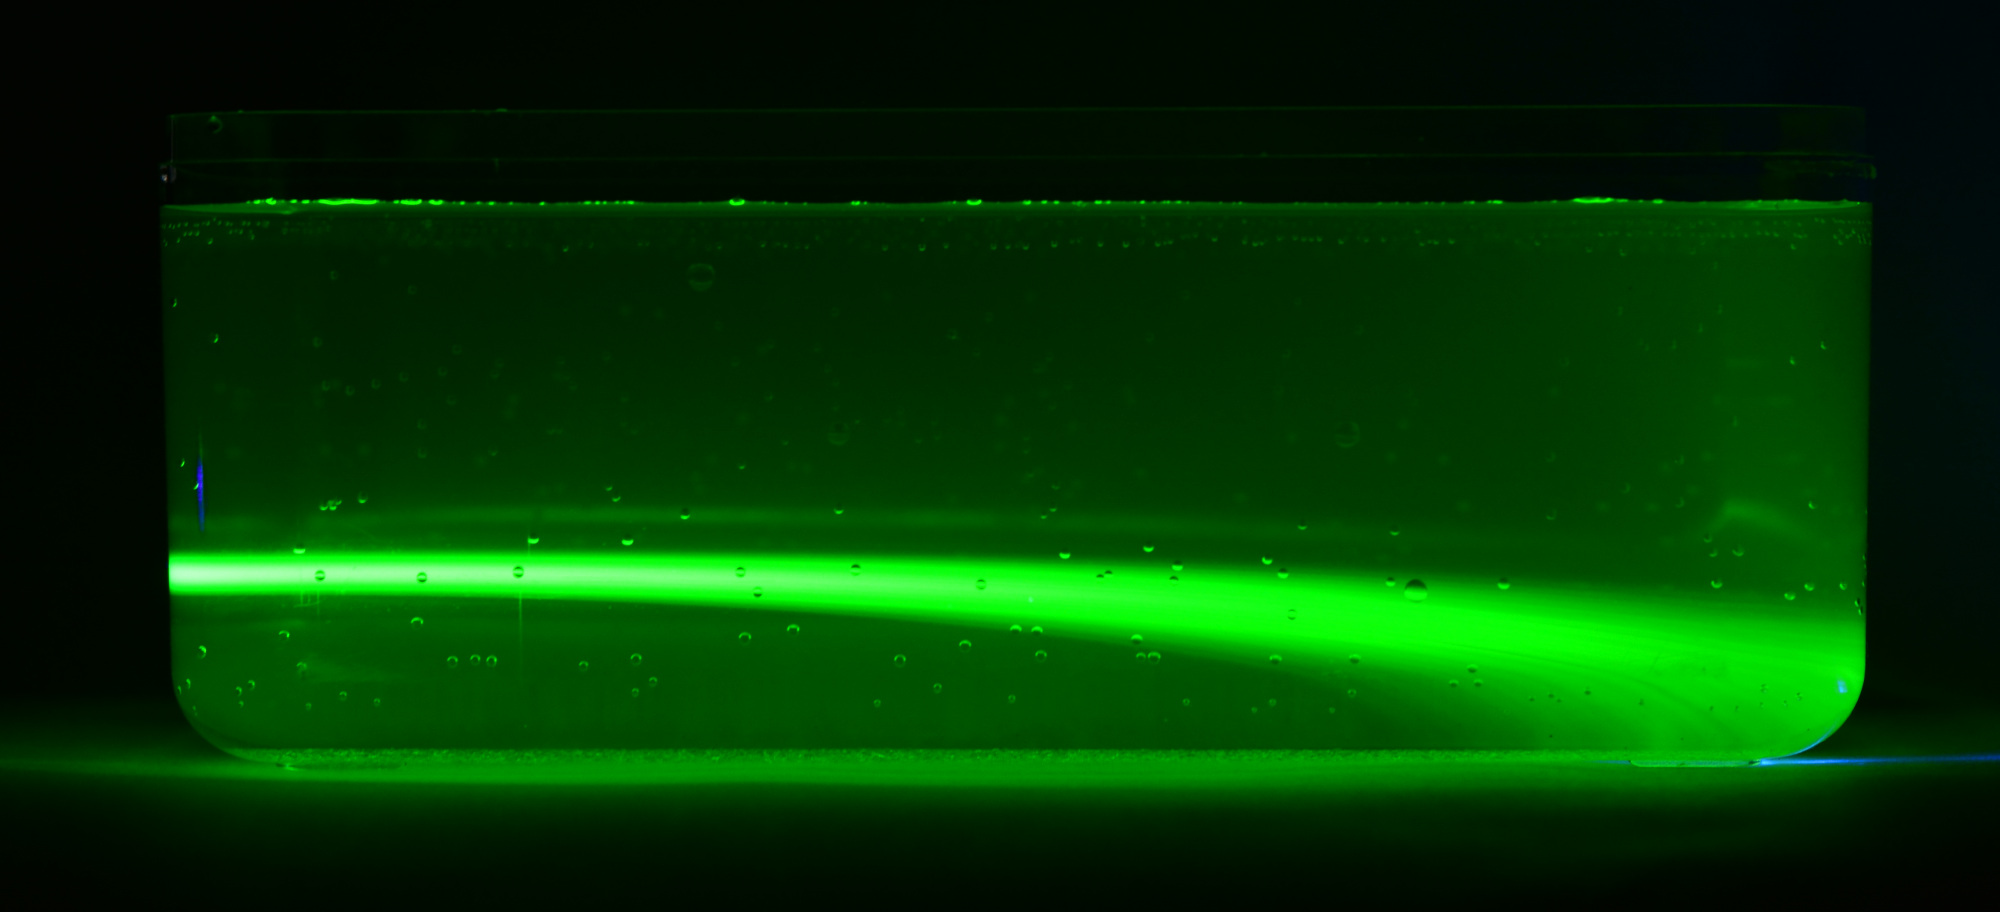
\includegraphics[width=10truecm]{slike/02_Sladkor.jpg}
\caption{Potek žarka v vodni raztopini sladkorja, v kateri koncentracija sladkorja in z
njo lomni količnik naraščata z globino. Vodi smo dodali fluorescein, da bolje vidimo potek žarka. Podobno se ukrivi potek žarka v neenakomerno segreti atmosferi, kar vodi
do pojava fatamorgane.}
\label{fig:02_Sladkor}
\end{figure}
\end{example}

\subsection*{Fatamorgana}
Ukrivljeno pot žarkov v snovi z nehomogenim lomnim količnikom opazimo
tudi v naravi. Kadar se tla (na primer asfaltna cesta) 
močno segrejejo, nastane nad njimi tanka plast zraka, ki je bistveno 
toplejši od zraka višje nad tlemi. Ali pa je tanka plast zraka nad 
hladnim morjem znantno hladnejša od toplega zraka v višjih legah. Ker je 
lomni količnik toplejšega zraka manjši od lomnega količnika hladnejšega zraka, 
se v obeh primerih pot svetlobe ukrivi, enkrat navzgor, drugič navzdol. Ta pojav
imenujemo zračno zrcaljenje ali fatamorgana. 

Spodnje zračno zrcaljenje nastopi, kadar je spodnja plast zraka toplejša 
od zgornjih plasti. Poglejmo, kako opazovalec vidi oddaljeno drevo 
(slika~\ref{fig:02_Fata1}). Od krošnje do opazovalca pridejo žarki
po razmeroma hladni plasti, hkrati pa pridejo do njega tudi žarki, ki 
se ukrivijo na močno segreti plasti zraka tik nad tlemi. Opazovalec
tako vidi dve sliki -- eno pravo in pod njo eno obrnjeno. Na enak način 
pojasnimo tudi odsev neba, ki ga pogosto vidimo na razgretih cestah.
Ker smo vajeni opazovati
odsev neba od vodne gladine, je vroča cesta videti mokra.
\begin{figure}[h!]
\centering
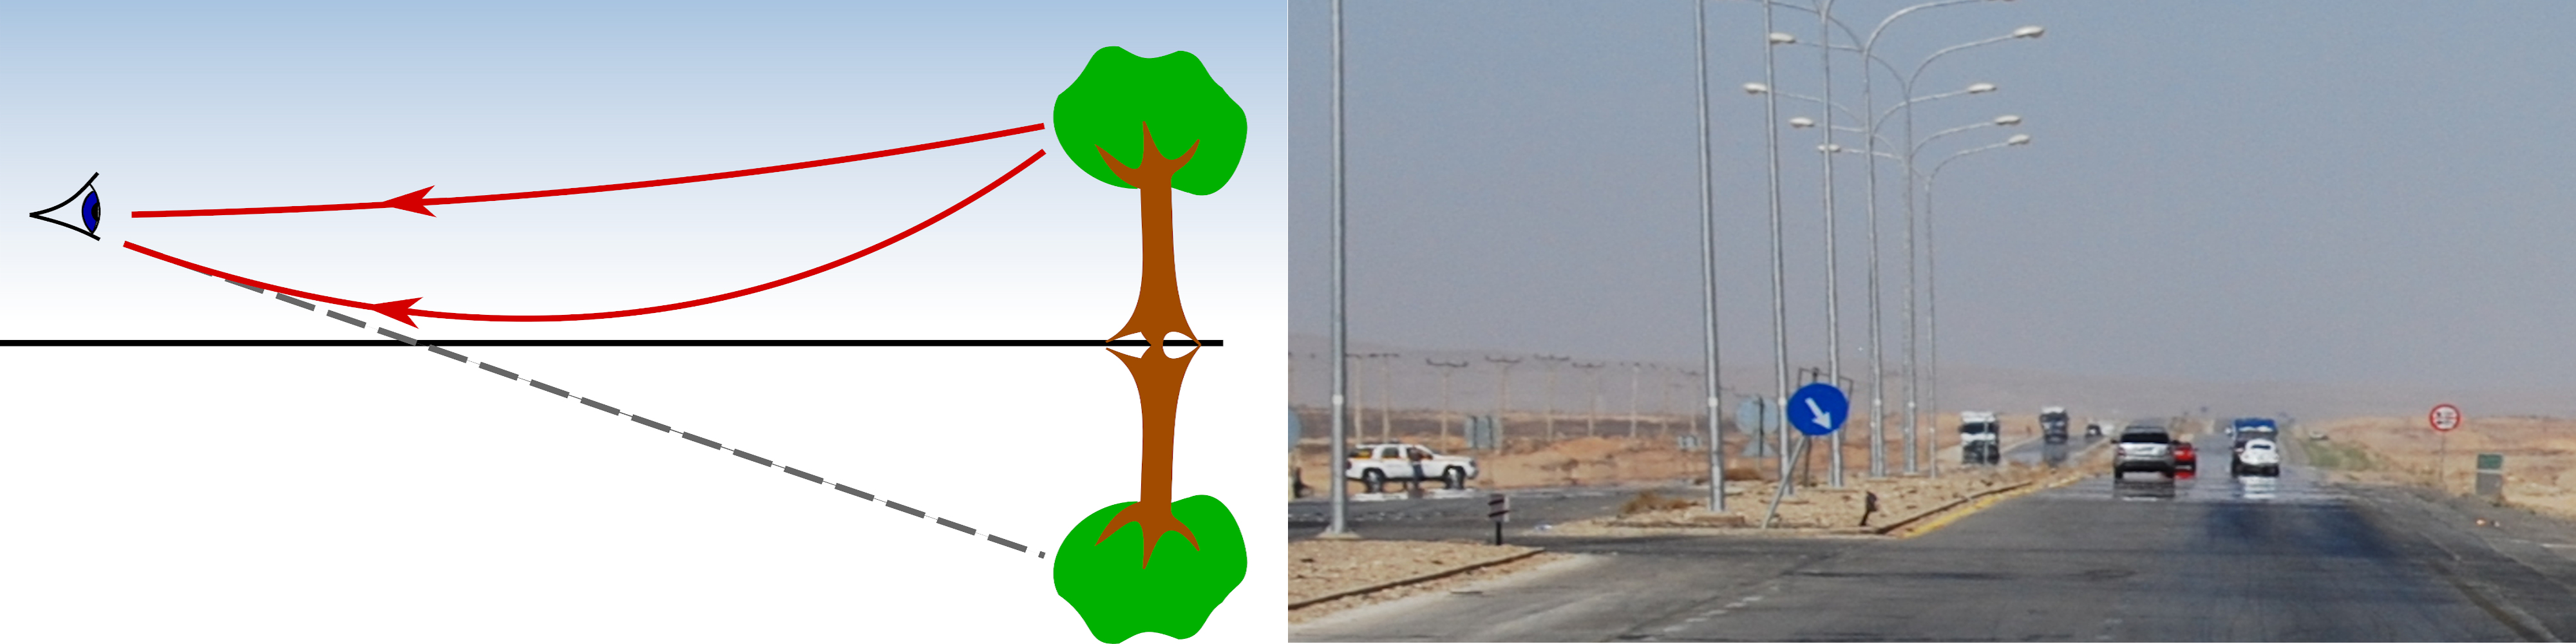
\includegraphics[width=12truecm]{slike/02_Fata1.jpg}
\caption{Zračno zrcaljenje na vročih tleh}
\label{fig:02_Fata1}
\end{figure}
\vglue-0.6truecm
Zgornje zračno zrcaljenje se nasprotno pojavi, 
kadar je spodnja plast zraka izrazito hladnejša od zgornjih plasti. 
Takrat se svetlobni žarki krivijo navzdol (slika~\ref{fig:02_Fata2})
in navidezno sliko predmeta premaknejo nad njegovo dejansko lego. 
Slika je lahko pokončna ali obrnjena, odvisno od oddaljenosti predmeta
in temperature plasti. 
\begin{figure}[h!]
\centering
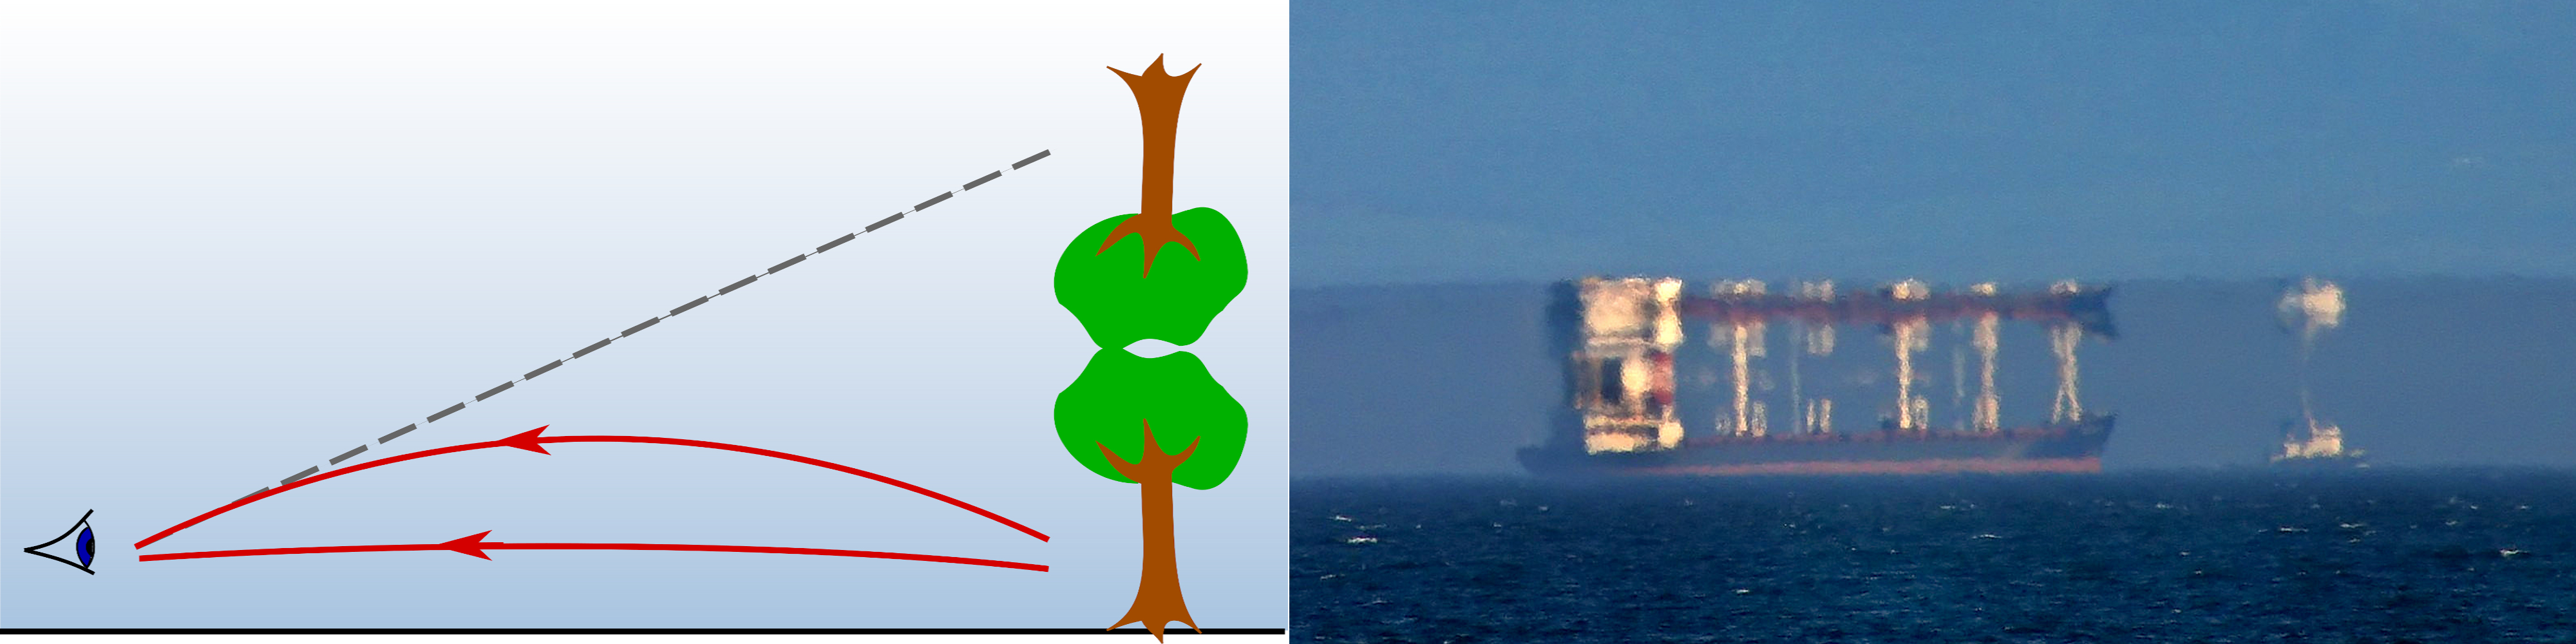
\includegraphics[width=12truecm]{slike/02_Fata2.jpg}
\caption{Zračno zrcaljenje na hladnejši podlagi (Foto: Craig Clements, Wikimedia)}
\label{fig:02_Fata2}
\end{figure}
\vglue-0.6truecm
Ukrivljena pot žarkov zaradi temperaturnega gradienta v atmosferi
vodi še do enega zanimivega pojava: popačenja oblike Sonca ob sončnem 
zahodu. Ker žarki s spodnjega dela Sonca potujejo po bolj ukrivljeni
poti kot žarki z zgornjega dela, se spodnji rob navidezno premakne navzgor 
in slika Sonca se splošči ali popači.
\begin{figure}[ht]
\centering
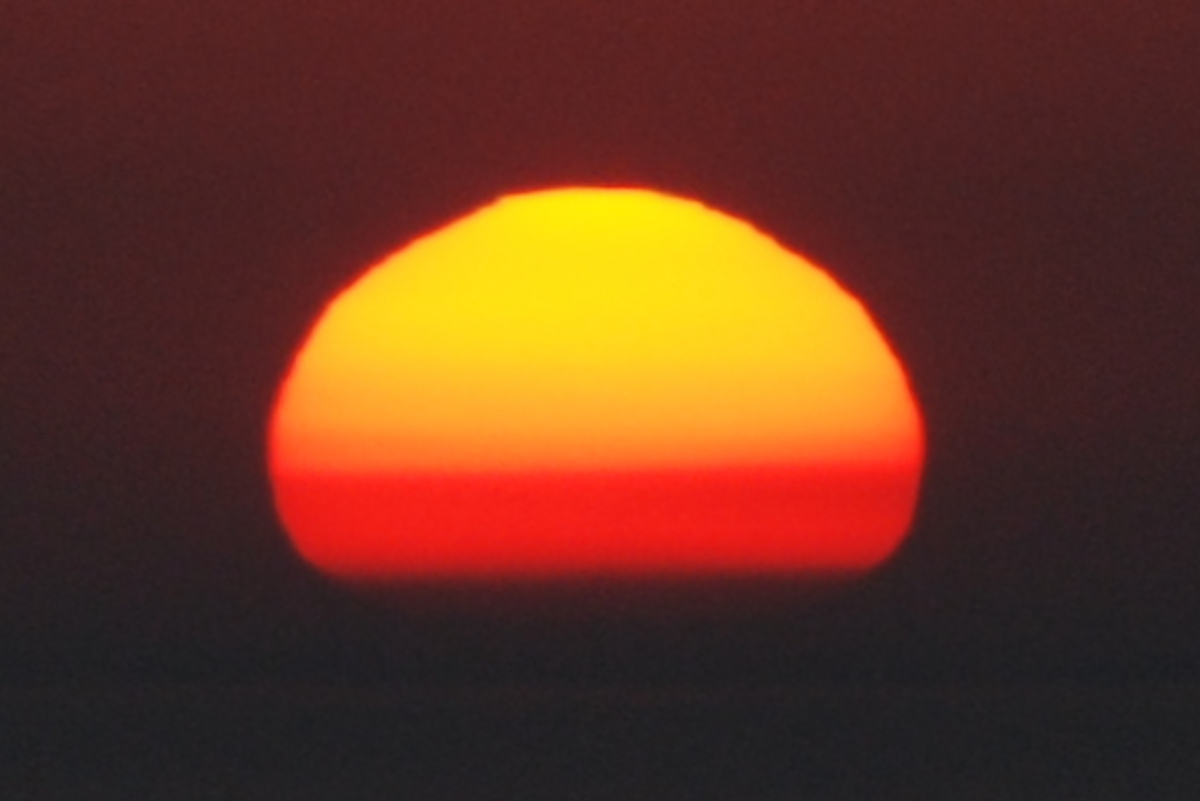
\includegraphics[width=5truecm]{slike/02_Sonce.jpg}
\caption{Sonce se ob sončnem zahodu navidezno splošči in njegova oblika popači.}
\label{fig:02_Sonce}
\end{figure}
\vglue-0.6truecm
\section{Transformacije žarkov z matrikami ABCD}
V prejšnjem razdelku smo zapisali žarkovno enačbo v obosnem 
približku (enačba~\ref{eq:02_24}). Ključna parametra za opis trajektorije žarka sta 
oddaljenost od optične osi $z$, ki jo označimo z $x$, in naklonski 
kot žarka glede na optično os, ki ga označimo s $\vartheta$.
Naša naloga je povezati dve točki žarka na različnih mestih v
prostoru in zapisati preslikavo med njima, če je med točkama
optični medij oziroma nek optični element. 
\begin{figure}[ht]
\centering
\def\svgwidth{90truemm} 
\input{slike/02_ABCD0.pdf_tex}
\caption{Pri danem $z$ žarek opišemo z lego $x$ in smerjo $\vartheta$. Spremembo
teh dveh parametrov opišemo s preslikavo.}
\label{fig:01_ABCD0}
\end{figure}

V splošnem vrednosti lege in naklona v točki 2 izrazimo kot 
linearno kombinacijo prvotnih vrednosti v točki 1:
\begin{align}
 x_2 &= A x_1 + B \vartheta_1 \qquad \mathrm{in}  \label{eq:02_29}\\
 \vartheta_2 &=  C x_1 + D\vartheta_1.
 \label{eq:02_30}
\end{align}
Če združimo parametra $x$ in $\vartheta$ v neki točki prostora
v dvodimenzionalni vektor,
lahko preslikavo strnjeno zapišemo v matrični obliki:
\boxeq{eq:02_31}{
\left[\begin{array}{c}
x_2\\
\vartheta_2
\end{array}\right] = 
\left[\begin{array}{cc}
A& B\\
C&D
\end{array}\right]
\left[\begin{array}{c}
x_1\\
\vartheta_1
\end{array}\right]
= M \left[\begin{array}{c}
x_1\\
\vartheta_1
\end{array}\right]\!\!.
}
Matriko $M$ imenujemo transformacijska oziroma prehodna matrika 
vmesnega optičnega medija ali optičnega elementa. 

\begin{example}
\label{ex:ML}
{\bf Matrika ABCD za premik v homogeni snovi s konstantnim lomnim količnikom.} 
Prvi primer naj bo homogena snov, v kateri je lomni količnik konstanten in enak $n$. 
V točki 1 pri $z_1$ naj bosta komponenti vektorja enaki $x_1$ in 
$\vartheta_1$. Poiščimo vrednosti komponent vektorja, 
če se premaknemo za $L$ vzdolž optične osi sistema do $z_2$ 
(slika~\ref{fig:01_ABCD1}). 
\begin{figure}[ht]
\centering
\def\svgwidth{70truemm} 
\input{slike/02_ABCD1.pdf_tex}
\caption{K izračunu matrike ABCD za premik v homogeni snovi}
\label{fig:01_ABCD1}
\end{figure}

Naklon žarka se pri premiku ne spremeni, zato ostane $\vartheta_2 = \vartheta_1$. Spremeni
pa se odmik od optične osi, saj žarek ne potuje vzporedno z osjo $z$. 
Vrednost $x_2$ zapišemo kot:
\begin{equation}
 x_2 = x_1 + (z_2-z_1)\vartheta_1 = x_1 + L\vartheta_1.
\label{eq:02_32}
\end{equation}
Potem zapišemo sistem enačb:
\begin{align}
 x_2 &= 1\cdot x_1 + L\cdot \vartheta_1 \qquad \mathrm{in} \label{eq:02_33}\\
 \vartheta_2 &= 0\cdot x_1 + 1\cdot \vartheta_1.
 \label{eq:02_34}
\end{align}
Iz zapisa razberemo koeficiente matrike $M$ za homogeno snov dolžine $L$:
\begin{equation}
 M = \left[\begin{array}{cc}
1& L\\
0&1
\end{array}\right]\!\!.
 \label{eq:02_35}
\end{equation}
\end{example}

\begin{example}
\label{ex:Mmeja}
{\bf Matrika ABCD za prehod skozi ravno mejo med dvema snovema.} Naj svetloba vpada na 
mejo dveh snovi z različnima lomnima količnikoma $n_1$ in $n_2$. Za izračun 
prehodne matrike izberemo dve točki na žarku: eno tik pred mejo in eno tik za njo. 
Lega žarka se ob tem ne spremeni in $x_2 = x_1$. 
Spremeni pa se naklon žarka. 
\begin{figure}[ht]
\centering
\def\svgwidth{70truemm} 
\input{slike/02_ABCD2.pdf_tex}
\caption{K izračunu matrike ABCD za prehod skozi ravno mejo med dvema snovema}
\label{fig:01_ABCD2}
\end{figure}

Za majhne naklone lahko lomni zakon
(enačba~\ref{eq:lomnizakon}) razvijemo in dobimo:
\begin{equation}
n_1 \vartheta_1 = n_2 \vartheta_2.
 \label{eq:02_36}
\end{equation}
Sistem enačb je potem:
\begin{align}
 x_2 &= 1\cdot x_1 + 0\cdot \vartheta_1 \qquad \mathrm{in} \label{eq:02_37}\\
 \vartheta_2 &= 0\cdot x_1 + \frac{n_1}{n_2}\cdot \vartheta_1.
 \label{eq:02_38}
\end{align}
Matrika $M$ za prehod skozi mejo med dvema snovema je:
\begin{equation}
 M = \left[\begin{array}{cc}
1& 0\\
0&\frac{n_1}{n_2}
\end{array}\right]\!\!.
\label{eq:02_39}
\end{equation}
\end{example}

\begin{example}
\label{ex:MUmeja}
{\bf Matrika ABCD za prehod skozi ukrivljeno mejo med dvema snovema.} V prejšnjem 
primeru je bila meja med snovema z lomnima količnikoma $n_1$ in $n_2$ ravna, zdaj pa 
poglejmo še matriko za prehod skozi ukrivljeno mejo. Krivinski radij mejne ploskve
naj bo $R$, pri čemer $R$ štejemo pozitivno, če je meja konveksna glede na smer
naraščajočega $z$ oziroma če je središče krožnice za mejo med snovema. V primeru, 
da je središče krožnice, ki določa mejo med snovema, pred mejo, je meja konkavna, 
krivinski radij mejne ploskve pa negativen. 

Za izračun matrike ponovno izberemo dve točki, prvo tik pred mejo in 
drugo tik za njo. To pomeni, da se oddaljenost od optične osi
pri prehodu ohranja in $x_1 = x_2$. 

Izračun naklona žarka po prehodu je malo bolj zapleten. Za zapis lomnega 
zakona moramo namreč vpeljati kote glede na normalo na
mejo. Vpadni kot je tako $\alpha = \vartheta_1 + \varphi$, lomni kot pa 
$\beta = \vartheta_2 + \varphi$ (glej sliko~\ref{fig:02_ABCD3}).
Privzamemo, da je ukrivljenost meje dovolj majhna oziroma da so žarki
dovolj blizu optične osi, da velja zveza:
\begin{equation}
 \sin \varphi = \frac{x_1}{R} \approx \varphi.
 \label{eq:02_40}
\end{equation}
\begin{figure}[!h]
\centering
\def\svgwidth{70truemm} 
\input{slike/02_ABCD3.pdf_tex}
\caption{K izračunu matrike ABCD za prehod skozi ukrivljeno mejo med dvema snovema}
\label{fig:02_ABCD3}
\end{figure}

Zapišemo lomni zakon,
pri čemer privzamemo, da so vsi koti majhni:
\begin{equation}
n_1 (\vartheta_1 + \varphi) = n_2 (\vartheta_2 + \varphi).
\label{eq:02_41}
\end{equation}
Od tod izračunamo kot $\vartheta_2$:
\begin{equation}
 \vartheta_2 = \frac{n_1-n_2}{n_2}\varphi + \frac{n_1}{n_2} \vartheta_1.
 \label{eq:02_42}
 \end{equation}
Če $\varphi$ izrazimo iz enačbe~(\ref{eq:02_40}), zapišemo transformacijo koordinat:
\begin{align}
 x_2 &= 1\cdot x_1 + 0\cdot \vartheta_1 \qquad \mathrm{in} \\
 \vartheta_2 &= \frac{n_1-n_2}{n_2R}\cdot x_1 + \frac{n_1}{n_2}\cdot \vartheta_1.
 \label{eq:02_43}
\end{align}
Razberemo matriko $M$ za prehod skozi ukrivljeno mejo med dvema snovema:
\begin{equation}
M = \left[\begin{array}{cc}
1& 0\\
\frac{n_1-n_2}{n_2R}&\frac{n_1}{n_2}
\end{array}\right]\!\!.
 \label{eq:02_44}
\end{equation}
V limitnem primeru, ko gre $R \to \infty$, se matrika prevede na matriko za
prehod skozi ravno mejo (glej primer~\ref{ex:Mmeja}).
\end{example}

Izračunajmo še determinanto izpeljanih matrik ABCD. Na splošno velja, da
je determinanta matrike ABCD enaka razmerju lomnih količnikov začetne in 
končne snovi. Če je lomni količnik snovi na koncu enak
kot na začetku (primer~\ref{ex:ML}), je $\det(M) = 1$, v nasprotnem primeru 
(primera~\ref{ex:Mmeja} in \ref{ex:MUmeja}) je $\det(M) = n_1/n_2$.

Do zdaj smo obravnavali matrike za posamezne prehode. Poglejmo, kako izračunamo
prehodno matriko za primer, če svetloba potuje skozi več elementov zapored. V tem
primeru se pokažeta izjemna praktičnost in uporabnost zapisa z matrikami, saj ob prehodu svetlobe skozi 
več elementov matrike za te elemente preprosto zmnožimo. Paziti moramo seveda
na vrsti red: matriko za element, na katerega vpade svetloba najprej, zapišemo
najbolj desno, to je najbliže vektorju, ki opisuje vpadno svetlobo. Celoten prehod
spet opiše ena sama matrika:
\begin{equation}
\left[\begin{array}{c}
x_N\\
\vartheta_N
\end{array}\right] 
= \tilde{M} \left[\begin{array}{c}
x_1\\
\vartheta_1
\end{array}\right]\!\!,
 \label{eq:02_45}
\end{equation}
pri čemer je:
\begin{equation}
\tilde{M} = M_N \cdot M_{N-1}~...~M_2 \cdot M_1.
 \label{eq:02_46}
\end{equation}
\begin{figure}[ht]
\centering
\def\svgwidth{100truemm} 
\input{slike/02_MMM.pdf_tex}
\caption{Prehod žarka skozi več optičnih elementov zapišemo kot produkt matrik posameznih prehodov.
Pri tem moramo paziti na vrstni red zapisa matrik.}
\label{fig:01_MMM}
\end{figure}

\section{Preslikave z lečami}
\label{chap:lecje}
Uporabimo matrike ABCD za izračun prehoda svetlobe skozi tanko lečo. Matriko
za prehod zapišemo kot produkt dveh matrik: prve, ki opiše
prehod skozi prvo ukrivljeno ploskev s krivinskim radijem $R_1$, 
in druge, ki opiše prehod skozi izhodno ukrivljeno ploskev s 
krivinskim radijem $R_2$. Za bikonveksno lečo, na primer, je 
$R_1>0$ in $R_2<0$ (glej sliko~\ref{fig:02_tankaleca}). 
Lomni količnik leče naj bo $n_2$ in snovi okoli leče 
(navadno je to zrak) $n_1$. Zanima nas, kako se vektor $(x_1, \vartheta_1)$ 
preslika v $(x_2, \vartheta_2)$.
\begin{figure}[!h]
\centering
\def\svgwidth{100truemm} 
\input{slike/02_tankaleca.pdf_tex}
\caption{K izračunu matrike ABCD za prehod skozi tanko bikonvkesno lečo}
\label{fig:02_tankaleca}
\end{figure}

Izračunajmo najprej matriko za prehod skozi lečo. Ker smo privzeli, da je leča tanka, 
vmesne matrike za premik po steklu ne zapišemo. Z upoštevanjem enačbe~(\ref{eq:02_44})
dobimo:
\beq
 M = \left[\begin{array}{cc}
1& 0\\
\frac{n_2-n_1}{n_1R_2}&\frac{n_2}{n_1}
\end{array}\right]\cdot 
\left[\begin{array}{cc}
1& 0\\
\frac{n_1-n_2}{n_2R_1}&\frac{n_1}{n_2}
\end{array}\right] = 
\left[\begin{array}{cc}
1& 0\\
\frac{n_2-n_1}{n_1}\left(\frac{1}{R_2}-\frac{1}{R_1}\right)&1
\end{array}\right]\!\!.
\label{eq:02_47}
\eeq
Vpeljemo parameter $f$, za katerega velja:
\beq
\frac{1}{f} = -\frac{n_2-n_1}{n_1}\left(\frac{1}{R_2}-\frac{1}{R_1}\right)\!\!.
\label{eq:02_48}
\eeq
Element matrike $C$ je tako enak $-1/f$. Fizikalni pomen tega parametra
bomo kmalu spoznali.

Uporabimo izračunano matriko za opis prehoda svetlobe skozi lečo. Naj žarek izhaja iz 
predmeta, ki je na oddaljenosti $a$ od leče, opazujemo pa ga na razdalji
$b$ za lečo. Za celotno pot žarka moramo zmnožiti tri matrike: matriko za 
premik do leče, matriko za prehod skozi lečo in matriko za premik do opazovalca.
Dobimo:
\beq
M = 
\left[\begin{array}{cc}
1& b\\
0&1
\end{array}\right]\cdot
\left[\begin{array}{cc}
1& 0\\
-\frac{1}{f}&1
\end{array}\right]
\cdot
\left[\begin{array}{cc}
1& a\\
0&1
\end{array}\right]
= 
\left[\begin{array}{cc}
1-\frac{b}{f}& a+b-\frac{ab}{f}\\
-\frac{1}{f}&1-\frac{a}{f}
\end{array}\right]\!\!.
\label{eq:02_49}
\eeq
Najprej poiščimo pomen parametra $f$, ki smo ga vpeljali z enačbo~(\ref{eq:02_48}).
Poglejmo, v kaj se preslikajo žarki, ki na neki oddaljenosti od osi $x_1$ vpadajo na lečo 
vzporedno z optično osjo $z$:
\beq
\left[\begin{array}{c}
x_2\\
\vartheta_2
\end{array}\right] =
\left[\begin{array}{cc}
1-\frac{b}{f}& a+b-\frac{ab}{f}\\
-\frac{1}{f}&1-\frac{a}{f}
\end{array}\right] \cdot
\left[\begin{array}{c}
x_1\\
0
\end{array}\right] = 
\left[\begin{array}{c}
\left(1-\frac{b}{f}\right)x_1\\
-\frac{x_1}{f}
\end{array}\right]\!\!.
\label{eq:02_51}
\eeq
Vsi vzporedni vpadni žarki se zberejo v eni točki, kadar velja $1-b/f = 0$ in $b=f$. 
Vzporedni žarki se torej zberejo na oddaljenosti $f$, zato 
parameter $f$ prestavlja goriščno razdaljo leče. 
Ker navadno obravnavamo lečo v zraku, enačbo~(\ref{eq:02_48}) za izračun 
goriščne razdalje leče poenostavljeno zapišemo  kot:
\boxeq{eq:goriscna}{
\frac{1}{f} = \left(n-1\right)\left(\frac{1}{R_1}-\frac{1}{R_2}\right)\!\!,
}
pri čemer je $n$ lomni količnik stekla, iz katerega je leča narejena, $R_1$ in $R_2$ pa 
sta krivinska radija mejnih ploskev leče.

Vrnimo se k izračunani matriki (enačba~\ref{eq:02_49}).
Da na desni strani leče nastane slika predmeta, se morajo 
žarki, ki izhajajo iz ene točke predmeta na levi, zbrati
v eni točki na desni strani leče, neodvisno od njihovega naklona.
Ta zahteva je izpolnjena le ob pogoju, da je element matrike prehoda $B = 0$ in velja:
\boxeq{eq:PreslikavaLeca}{
\frac{1}{f} = \frac{1}{a}+\frac{1}{b}.
}
Dobili smo enačbo leče, ki povezuje lego predmeta z lego njegove slike.

Razmerje med velikostima slike $x_2$ in predmeta $x_1$ določa
element matrike $A$, ki ga z upoštevanjem enačbe~(\ref{eq:PreslikavaLeca})
zapišemo kot:
\beq
A= 1-\frac{b}{f} = 1 - b\left(\frac{1}{a}+\frac{1}{b}\right) = -\frac{b}{a}.
\label{eq:02_50}
\eeq
Povečava leče je tako enaka:
\boxeq{eq:PovecavaLece}{
\frac{x_2}{x_1} =-\frac{b}{a}.
}
Negativni predznak pomeni, da je slika predmeta desno od leče obrnjena na glavo
(glej sliko~\ref{fig:02_slikazaleco}).
\begin{figure}[!ht]
\centering
\def\svgwidth{140truemm} 
\input{slike/02_slikazaleco.pdf_tex}
\caption{Kadar je predmet bolj oddaljen od leče kot je goriščna razdalja ($a>f$),
nastane obrnjena prava slika desno od leče. 
V tem primeru sta $a,b>0$ (levo). Če je predmet blizu leče in velja $a<f$,
nastane pokončna navidezna slika na isti strani, kot je predmet. V tem primeru velja $a>0$ in $b<0$.}
\label{fig:02_slikazaleco}
\end{figure}

Če je predmet oddaljen od leče več kot je goriščna razdalja, nastane na desni
strani na glavo obrnjena prava slika, ki jo lahko projiciramo na zaslon. Če je 
predmet blizu leče in velja $a<f$, je po enačbi~(\ref{eq:PreslikavaLeca}) 
vrednost $b$ negativna. Žarki desno od leče se ne sekajo, temveč se sekajo podaljški 
žarkov levo od leče. Slika predmeta je tako le navidezna in je
ne moremo projicirati na zaslon. Povečava take slike je pozitivna, 
kar pomeni, da je navidezna slika pokončno obrnjena.

Opisani izračun je bil narejen na primeru bikonveksne leče, vendar velja
povsem splošno za poljubno tanko lečo. Paziti moramo le na predznake krivinskih
radijev vstopne in izstopne ploskve. Če je ena stranica leče ravna, je 
njen krivinski radij neskončen. 

\begin{example}{\bf Preslikava z dvema zaporednima lečama.}
Poglejmo prehod svetlobe skozi dve zaporedni tanki leči z goriščnima
razdaljama $f_1$ in $f_2$, ki sta na medsebojni oddaljenosti $s$.
\begin{figure}[!h]
\centering
\def\svgwidth{100truemm} 
\input{slike/02_dveleci.pdf_tex}
\caption{Prehod svetlobe skozi sistem dveh tankih leč}
\label{fig:02_lecje}
\end{figure}

Matriko sistema dveh leč za prehod z leve proti desni zapišemo kot:
\beq
M = 
\left[\begin{array}{cc}
1& 0\\
-\frac{1}{f_2}&1
\end{array}\right]\cdot 
\left[\begin{array}{cc}
1& s\\
0&1
\end{array}\right]\cdot
\left[\begin{array}{cc}
1& 0\\
-\frac{1}{f_1}&1
\end{array}\right] = 
\left[\begin{array}{cc}
1-\frac{s}{f_1}& s\\
-\frac{1}{f_1}-\frac{1}{f_2}+\frac{s}{f_1f_2}&1-\frac{s}{f_2}
\end{array}\right]\!\!.
\label{eq:02_54}
\eeq
Izračunajmo goriščno razdaljo takega sistema in lego gorišča
na desni strani. Za opis  žarkov desno
od sistema je treba matriko prehoda pomnožiti še z matriko premika za $d$. 

Naj bodo vpadni žarki vzporedni z optično osjo in jih zapišemo 
v obliki vektorja $(x_1,0)$. Izhodne žarke potem izračunamo kot:
\beq
\left[\begin{array}{c}
x_2\\
\vartheta_2
\end{array}\right]
 = 
\left[\begin{array}{cc}
1& d\\
0&1
\end{array}\right]
\cdot
\left[\begin{array}{cc}
A& B\\
C&D
\end{array}\right]\cdot 
\left[\begin{array}{c}
x_1\\
0
\end{array}\right] = 
\left[\begin{array}{c}
\left(A+dC\right)x_1\\
Cx_1
\end{array}\right]\!\!,
\label{eq:02_55}
\eeq
pri čemer so elementi matrike ABCD podani z enačbo~(\ref{eq:02_54}). 
Po definiciji se vzporedni vpadni žarki po prehodu sekajo v gorišču, 
zato je naklon izhodnega žarka $\vartheta_2 = -x_1/f$ in $C = -1/f$. 
Od tod razberemo goriščno razdaljo sistema:
\boxeq{eq:lecje}{
\frac{1}{f} = \frac{1}{f_1} + \frac{1}{f_2} - \frac{s}{f_1f_2}.
}
Oddaljenost gorišča od desne leče določimo iz pogoja, da je v gorišču $x_2 = 0$. Dobimo:
\beq
d = -\frac{A}{C} = \frac{f_1f_2-sf_2}{f_1+f_2-s}.
\label{eq:02_56}
\eeq
Pri sestavu leč pogosto vpeljemo glavno ravnino. To je ravnina, pravokotna
na optično os, v kateri bi 
bila postavljena nadomesta tanka leča. Dobimo jo tako, da poiščemo 
presečišče žarkov, ki vpadajo na sistem vzporedno z optično osjo, 
in žarkov ali njihovih podaljškov, ki iz sestava izhajajo desno od lečja. 
Ko poznamo lego gorišča, je lego glavne ravnine preprosto določiti, 
saj vemo, da je glavna ravnina od gorišča oddaljena ravno za goriščno razdaljo.

Račun je bil narejen za prehod svetlobe iz
leve proti desni strani. Ker se leči v splošnem razlikujeta in matrike
ne komutirajo, je prehod z desne proti levi drugačen. Skupna goriščna
razdalja ostane enaka, premakneta pa se lega gorišča in glavna ravnina.
\end{example}

\begin{example}{\bf Preslikava z debelo lečo}
Matriko za prehod skozi debelo lečo s krivinskima radijema
$R_1$ in $R_2$ ter debelino $d$ lahko neposredno izračunamo
z množenjem treh matrik: matrike za prehod skozi ukrivljeno vstopno 
ploskev, matrike za premik znotraj leče in matrike za prehod skozi 
ukrivljeno izstopno ploskev, pri čemer naj bo $n_1 = 1$:
\beq
M = 
\left[\begin{array}{cc}
1& 0\\
\frac{n-1}{R_2}&n
\end{array}\right]
\cdot
\left[\begin{array}{cc}
1& d\\
0&1
\end{array}\right]
\cdot
\left[\begin{array}{cc}
1& 0\\
\frac{1-n}{nR_1}&\frac{1}{n}
\end{array}\right]\!\!.
\label{eq:02_52}
\eeq
Matriko za prehod lahko izračunamo tudi drugače, na podlagi podobnosti 
s sistemom dveh leč. Debelo lečo razdelimo
na tri dele: vstopno plankonveksno lečo, plast stekla in izstopno plankonkavno lečo.
Goriščni razdalji leč zapišemo z uporabo enačbe~(\ref{eq:goriscna}), pri čemer upoštevamo, 
da je krivinski radij ravne stranice neskončen:
\beq
\frac{1}{f_1} = (n-1)\frac{1}{R_1}\qquad \mathrm{in} \qquad \frac{1}{f_2} = -(n-1)\frac{1}{R_2}.
\label{eq:02_53}
\eeq
Pri vmesnemu prehodu skozi steklo moramo upoštevati tudi njegov
lomni količnik. Na splošno se pri prehodu žarka skozi plast snovi debeline $d$
z lomnim količnikom $n$ matrika zapiše kot:
\beq
M = 
\left[\begin{array}{cc}
1& 0\\
0&n
\end{array}\right]\cdot
\left[\begin{array}{cc}
1& d\\
0&1
\end{array}\right]\cdot
\left[\begin{array}{cc}
1& 0\\
0&\frac{1}{n}
\end{array}\right] = 
\left[\begin{array}{cc}
1& \frac{d}{n}\\
0&1
\end{array}\right]\!\!.
\label{eq:02_54a}
\eeq
Efektivna dolžina poti skozi snov je torej skrajšana za faktor $n$.

Ugotovitve vstavimo v enačbo za lečje (enačba~\ref{eq:02_54}) in dobimo:
\beq
M = 
\left[\begin{array}{cc}
1-\frac{d}{nf_1}& \frac{d}{n}\\
-\frac{1}{f_2}-\frac{1}{f_1}+\frac{d}{nf_1f_2}&1-\frac{d}{nf_2}
\end{array}\right]\!\!.
\label{eq:02_53a}
\eeq
Hitro lahko preverimo, da dobimo isti rezultat, če zmnožimo matrike v enačbi~(\ref{eq:02_52}).
Prav tako hitro preverimo tudi, da je izračunana matrika za debelo lečo v limitnem 
primeru $d \to 0$ enaka matriki za prehod skozi tanko lečo. 
\end{example}

\begin{remark}
Vsi izračuni so bili narejeni v obosnem 
približku, v katerem je smer žarka le malo odstopala od smeri optične osi. V praksi se lahko 
zgodi, da ta pogoj ni izpolnjen in preslikani žarki se ne sekajo v isti točki. Ta pojav opišemo
kot napako leče. Poleg navedenega je še vrsta drugih razlogov, na primer nepravilnost leče 
ali odvisnost lomnega količnika leče od valovne dolžine, ki vodijo do popačenja slike. 
Marsikatero od teh nepravilnost lahko odpravimo tako, da namesto ene same leče uporabimo 
zapleten sestav leč, ki deluje podobno kot ena idealna leča. Fotografski objektivi so 
tako navadno sestavljeni iz vsaj treh do štirih leč, zapletenejši tudi več kot petnajstih.
\end{remark}
 
\section{Odboj svetlobe na zrcalih}
Opis odboja na ravnih zrcalih je 
preprost: vse slike posamezne točke se po odboju zberejo v eni točki, 
navidezna slika, ki pri tem nastane, pa je enako velika in enako obrnjena kot predmet.
Matrika ABCD, ki opiše odboj od takega zrcala, je identiteta. Pri tem se moramo
zavedati, da žarek po odboju spremeni smer in z njim tudi os $z$.

Poiščimo še matriko za odboj od ukrivljenega zrcala. Naj bo krivinski radij zrcala
$R$, pri čemer za konkanvna zrcala, pri katerih sta predmet in krivinsko središče
na isti strani zrcala, velja $R>0$. Pri odboju na zrcalu se lega žarka ne spremeni, zato 
je $x_2 = x_1 = x$. Od tod takoj izračunamo prva dva elementa matrike ABCD: $A = 1$ in 
$B=0$. Pri transformaciji kota si pomagamo s sliko~\ref{fig:02_zrcalo}. 
\begin{figure}[!h]
\centering
\def\svgwidth{80truemm} 
\input{slike/02_zrcalo.pdf_tex}
\caption{K izračunu matrike ABCD za odboj na kroglastem zrcalu}
\label{fig:02_zrcalo}
\end{figure}

Naj bo $\alpha$ kot med optično osjo in zveznico med središčem krožnice in točko, 
v kateri vpada žarek na zrcalo. Vpadni žarek naj se širi pod kotom $\vartheta_1$, tako da
je vpadni kot glede na normalo na zrcalo enak $\alpha -\vartheta_1$. Kot, pod katerim 
se žarek odbije glede na vodoravnico naj bo $-\vartheta_2$, tako da je odbojni kot glede
na normalo na zrcalo enak $\vartheta_2 - \alpha$. Po odbojnem zakonu sta vpadni in odbojni
kot enaka, zato:
\beq
\alpha - \vartheta_1= \vartheta_2-\alpha.
\label{eq:02_60}
\eeq
Za majhne vrenosti velja $\alpha \approx x/R$, od koder sledi:
\beq
-\vartheta_2 = \vartheta_1 - \frac{2}{R}x.
\label{eq:02_61a}
\eeq
Od tod lahko razberemo elementa matrike $C = -2/R$ in $D = 1$. Celotna matrika za odboj 
na zrcalu je potem:
\begin{equation}
 M = \left[\begin{array}{cc}
1& 0\\
-\frac{2}{R}&1
\end{array}\right]\!\!.
 \label{eq:02_62}
\end{equation}
Naj žarek vpada na zrcalo v smeri vzporedno z optično osjo $(x_1, 0)$:
\begin{equation}
\left[\begin{array}{c}
x_2\\
\vartheta_2
\end{array}\right]
= \left[\begin{array}{cc}
1& 0\\
-\frac{2}{R}&1
\end{array}\right]\cdot
\left[\begin{array}{c}
x_1\\
0
\end{array}\right] = 
\left[\begin{array}{c}
x_1\\
-\frac{2x_1}{R}
\end{array}\right]\!\!.
 \label{eq:02_63}
\end{equation}
Žarek tik po odboju svoje lege ne spremeni, spremeni pa svojo smer.
Ker je usmerjen proti gorišču, je podobno kot
pri obravnavi leče njegova smer $\vartheta_2 = -x_1/f$. 
Od tod razberemo goriščno razdaljo krogelnega zrcala kot:
\boxeq{eq:02_zrcalof}{
f = \frac{R}{2}.
}
Preslikajmo še poljuben predmet, ki je na razdalji $a$ od temena zrcala, in poiščimo
pogoj za nastanek njegove slike na mestu $b$:
\beq
M = 
\left[\begin{array}{cc}
1& b\\
0&1
\end{array}\right]\cdot
\left[\begin{array}{cc}
1& 0\\
-\frac{2}{R}&1
\end{array}\right]
\cdot
\left[\begin{array}{cc}
1& a\\
0&1
\end{array}\right]
= 
\left[\begin{array}{cc}
1-\frac{2b}{R}& a+b-\frac{2ab}{R}\\
-\frac{2}{R}&1-\frac{2a}{R}
\end{array}\right]\!\!.
\label{eq:02_64}
\eeq
Da po odboju nastane ostra slika predmeta, mora biti element matrike $B=0$ 
(glej enačbo~\ref{eq:PreslikavaLeca}). To velja, kadar je izpolnjen pogoj:
\boxeq{eq:PreslikavaZrcalo}{
\frac{1}{f} = \frac{2}{R} = \frac{1}{a}+\frac{1}{b}.
}
Pri konkavnem zrcalu je $R>0$, vrednosti $a$ in $b$ pa sta pozitivni, če sta 
na isti strani kot krivinsko središče. Če je predmet od zrcala oddaljen več 
kot gorišče, je njegova slika prava in obrnjena. Vrednost $b$ je v tem primeru pozitivna.
Za predmete, za katere velja $a<f$, se odbiti žarki ne sekajo. Narisati
moramo podaljške žarkov in slika nastane na mestu, kjer se sekajo podaljški odbitih
žarkov (slika~\ref{fig:02_zrcaloodboj}).
\begin{figure}[!ht]
\centering
\def\svgwidth{140truemm} 
\input{slike/02_zrcaloodboj.pdf_tex}
\caption{Kadar je predmet bolj oddaljen od zrcala kot je goriščna razdalja ($a>f$),
nastane na isti strani zrcala obrnjena prava slika. 
V tem primeru sta $a,b>0$ (levo). Če je predmet blizu zrcala in velja $a<f$,
nastane pokončna navidezna slika na drugi strani zrcala. V tem primeru velja $a>0$ in $b<0$.}
\label{fig:02_zrcaloodboj}
\end{figure}

Povsem enako kot pri lečah izračunamo tudi povečavo zrcala. Element matrike $A$
preoblikujemo z upoštevanjem enačbe~(\ref{eq:PreslikavaZrcalo}) in dobimo:
\boxeq{eq:PovecavaZrcala}{
\frac{x_2}{x_1} =-\frac{b}{a}.
}
Gornji izračun je bil narejen na primeru konkavnega zrcala. Vendar so rezultati
povsem splošni in veljajo za vsa ukrivljena zrcala, pri čemer
je krivinski radij konveksnih zrcal negativen, ravnih zrcal pa neskončen. 

Z vpeljavo matrike za preslikavo z zrcalom lahko na preprost način v izračun
poti žarka v obosnem približku vključimo tudi zrcala. Vendar ne pozabimo, da se
pri odboju na zrcalu spremeni smer optične osi, kar moramo upoštevati v nadaljnjem računu.

\section{Preproste optične naprave}
Za konec si oglejmo še delovanje nekaterih optičnih naprav. Obravnavali jih bomo 
v najpreprostejši, a zato najnazornejši obliki. Izhajamo iz sestava dveh leč, ki 
smo jih obravnavali v razdelku~\ref{chap:lecje}. 

\subsection*{Razširjevalec snopov}
Spomnimo se matričnega zapisa prehoda skozi sistem dveh leč z goriščnima razdaljama
$f_1$ in $f_2$, ki sta na medsebojni razdalji $s$ (enačba~\ref{eq:02_54}). Poiščimo
pogoj, pri katerem so tako vpadni kot izhodni žarki iz sistema vzporedni z optično osjo.
Da je ta pogoj izpolnjen pri vseh vstopnih $x$, mora biti 
element prehodne matrike $C$ enak nič:
\beq
C = -\frac{1}{f_1}-\frac{1}{f_2} + \frac{s}{f_1f_2} = 0,
\label{eq:02_65}
\eeq
od koder sledi:
\beq
s = f_1 + f_2.
\label{eq:02_57}
\eeq
Vzporedni vpadni žarki izhajajo kot vzporedni žarki, kadar goriščni ravnini leč sovpadata.
Povečava takega sistema je z upoštevanjem enačbe~(\ref{eq:02_57}) enaka:
\beq
\frac{x_2}{x_1} = A = 1 - \frac{s}{f_1} = \frac{f_2}{f_1}.
\label{eq:02_58}
\eeq
Če je goriščna razdalja druge leče večja od goriščne razdalje prve leče, 
lahko širino snopa vzporednih vpadajočih žarkov močno povečamo -- žarek razširimo.
Tako napravo zato imenujemo razširjevalec snopov in je zelo uporabna v optičnih laboratorijih.

\subsection*{Teleskop in daljnogled}
Teleskop in daljnogled uporabljamo za opazovanje zelo oddaljenih predmetov, 
zato lahko privzamemo, da vpadajo žarki s teh predmetov na optični sistem praktično vzporedno. 
Naj bo zorni kot, pod katerim vidimo oddaljen predmet brez teleskopa, enak $\vartheta_1$.
Da so vzporedni tudi izhodni žarki, uporabimo lečje, pri katerem je razdalja med 
lečama enaka vsoti goriščnih razdalj obeh leč. Vstopno lečo imenujemo objektiv, 
izstopno lečo pa okular. Pravo sliko, ki nastane po prehodu objektiva,
opazujemo z okularjem, nastala slika pa je v tej preprosti izvedbi obrnjena. 
\begin{figure}[ht]
\centering
\def\svgwidth{100truemm} 
\input{slike/02_teleskop.pdf_tex}
\caption{V preprostem teleskopu gorišči leč sovpadata. V goriščni ravnini nastane 
slika predmeta, ki jo opazujemo z okularjem.}
\label{fig:02_teleskop}
\end{figure}
\vglue-10truemm
Poiščimo še povečavo takega preprostega teleskopa. Vpadni žarek, ki gre skozi središče
objektiva, je enak $(0,\vartheta_1)$. Izračunajmo izhodni žarek po prehodu skozi 
optični sistem, ki ga v splošnem opisuje matrika (enačba~\ref{eq:02_54}). Dobimo:
\beq
\left[\begin{array}{c}
x_2\\
\vartheta_2
\end{array}\right] = 
\left[\begin{array}{cc}
1-\frac{f_1+f_2}{f_1}& f_1+f_2\\
-\frac{1}{f_1}-\frac{1}{f_2}+\frac{f_1+f_2}{f_1f_2}&1-\frac{f_1+f_2}{f_2}
\end{array}\right] 
\cdot
\left[\begin{array}{c}
0\\
\vartheta_1
\end{array}\right]  = 
\left[\begin{array}{c}
(f_1+f_2) \vartheta_1\\
-\frac{f_1}{f_2}\vartheta_1
\end{array}\right]\!\!.
\label{eq:02_66}
\eeq
Zorni kot, pod katerim vidimo izhodne žarke $\vartheta_2$ je enak vstopnemu zornemu kotu, 
pomnoženemu z razmerjem goriščnih razdalj leč:
\boxeq{eq:teleskop}{
\vartheta_2 = -\frac{f_1}{f_2}\vartheta_1.
}
Če je goriščna razdalja objektiva $f_1$ večja
od goriščne razdalje okularja $f_2$, vidimo oddaljen predmet povečan.
Negativni predznak pri razmerju pomeni, da vidimo sliko obrnjeno na glavo. 

V praksi so teleskopi sestavljeni precej bolj zapleteno. Lahko so sestavljeni iz kombinacije
konveksnih in konkavnih leč, skoraj vedno pa vsebujejo tudi zrcala, saj je izdelava
velikih ukrivljenih zrcal preprostejša od izdelave velikih leč. 

\subsection*{Mikroskop}
Za opazovanje majhnih predmetov uporabimo mikroskop. Preprost mikroskop je sestavljen
iz dveh leč: objektiva, ki je bliže predmetu, in okularja, ki je bliže očesu 
(slika~\ref{fig:02_mikroskop}). Obe leči 
naj bosta zbiralni z goriščnima razdaljama $f_1$ in $f_2$ na oddaljenosti $s$. Predmet
postavimo blizu objektivu, vendar dovolj daleč, da velja $a>f_1$. Za objektivom 
nastane prava, povečana in obrnjena slika predmeta. Nastalo sliko opazujemo z okularjem, 
tako da so izhodni žarki praktično vzporedni in izhajajo iz sistema pod kotom $\vartheta_2$.
\begin{figure}[ht]
\centering
\def\svgwidth{100truemm} 
\input{slike/02_mikroskop.pdf_tex}
\caption{Preprost mikroskop je sestavljen iz dveh leč. Predmet je blizu objektivu, sliko
predmeta opazujemo z okularjem.}
\label{fig:02_mikroskop}
\end{figure}

Izračunajmo še povečavo preprostega mikroskopa, sestavljena iz dveh zbiralnih leč. Izhajamo
iz matrike za prehod skozi lečje (enačba~\ref{eq:02_54}). Vstopni žarek izberemo vzporeden
z optično osjo $(x_1, 0)$, izhodni pa naj bo $(0, \vartheta_2)$. Dobimo:
\beq
\left[\begin{array}{c}
0\\
\vartheta_2
\end{array}\right] = 
\left[\begin{array}{cc}
1-\frac{s}{f_1}& s\\
-\frac{1}{f_1}-\frac{1}{f_2}+\frac{s}{f_1f_2}&1-\frac{s}{f_2}
\end{array}\right] 
\cdot
\left[\begin{array}{c}
x_1\\
0
\end{array}\right]  = 
\left[\begin{array}{c}
\left(1-\frac{s}{f_1}\right)x_1\\
\left(\frac{s}{f_1f_2}-\frac{1}{f_1}-\frac{1}{f_2}\right)x_1
\end{array}\right]\!\!.
\label{eq:02_67}
\eeq
Vpeljemo $d$ kot razdaljo med notranjimi gorišči mikroskopa
$d= s -f_1-f_2$ in izračunamo zorni kot, pod katerim opazujemo predmet:
\beq
\vartheta_2 = \frac{x_1 d}{f_1f_2}.
\label{eq:02_69}
\eeq
Povečavo mikroskopa vpeljemo glede na zorni kot, pod katerim 
normalno vidimo predmet s prostim očesom, to je:
\beq
\vartheta_0 = \frac{x_1}{a_0},
\label{eq:02_70}
\eeq
pri čemer je po dogovoru normalna vidna razdalja $a_0 = 25~\si{cm}$.
Povečava mikroskopa je potem razmerje zornih kotov:
\beq
\frac{\vartheta_2}{\vartheta_0} = \frac{a_0d}{f_1f_2}.
\eeq

\subsection*{Oko in korekcijska očala}
Človeško oko ima na vstopni strani bikonveksno lečo, ki vpadno 
svetlobo zbere na mrežnici na zadnji strani očesa. 
Goriščna razdalja očesne leče je spremenljiva, da se lahko 
prilagaja za opazovanje tako bližnjih kot oddaljenih
predmetov. 

Če slika predmeta, ki nastane po prehodu skozi očesno lečo,
ne nastane točno na mrežnici, oseba za oster vid potrebuje korekcijska očala.
Daljnovidnost nastopi, kadar slika preslikanih predmetov nastane
za mrežnico. Oseba oddaljene predmete vidi ostro, očesna leča 
pa ne more imeti dovolj kratke goriščne razdalje, da bi nastala ostra 
slika predmetov, ki so na majhnih oddaljenostih od očesa. Vid popravimo z očali z 
zbiralno lečo. Po drugi strani pri kratkovidnih osebah slika
oddaljenih predmetov nastane pred mrežnico, saj očesna leča 
ne more doseči dovolj velikih goriščnih razdalj. Vid popravimo
z razpršilno lečo. 

\begin{remark}
 Kadar govorimo o vidu in korekcijskih očalih, navadno vpreljemo
 še eno praktično fizikalno količino. Namesto goriščne razdalje
 leče $f$ vpeljemo inverzno goriščno razdaljo, ki jo imenujemo 
 lomnost $\mathcal{D}$. Ker smo pri sestavu leč seštevali inverzne
 vrednosti goriščnih razdalj, lomnost leč preprosto seštejemo. 
 Enota za lomnost je dioptrija, pri čemer velja $1~\mathrm{dioptrija} = 
 1~\si{m}^{-1}$.
\end{remark}

\section{Primeri leč in zrcal}
Poglejmo nekaj primerov leč in zrcal, ki jih srečujemo v vsakdanu. Zbiralne leče
(navadno bikonveksne) uporabljamo kot lupe za povečavo pri branju ali 
natančnem delu. Kot zbiralna leča delujejo tudi kapljice vode, okrogli 
kozarci, napolnjeni z vodo, ali steklene krogle. Posebej zanimive so zbiralne leče
v svetilnikih, ki svetlobo z majhnega svetila preslikajo v vzporeden snop svetlobe, ki 
je viden od zelo daleč. Ker bi bile navadne plankonveksne leče prevelike in pretežke, se
v svetilnikih uporablja tako imenovane Fresnelove leče. Sestavljene
so iz kolobarjev, ki imajo enako ukrivljenost kot navadna leča, le da so bistveno
tanjši in zato leča lažja. Razpršilne leče se med drugih uporabljajo v vratnih kukalih. 

\begin{figure}[ht]
\centering

\includegraphics[width=7truecm]{slike/02_photos_lupa.jpg}\hfill
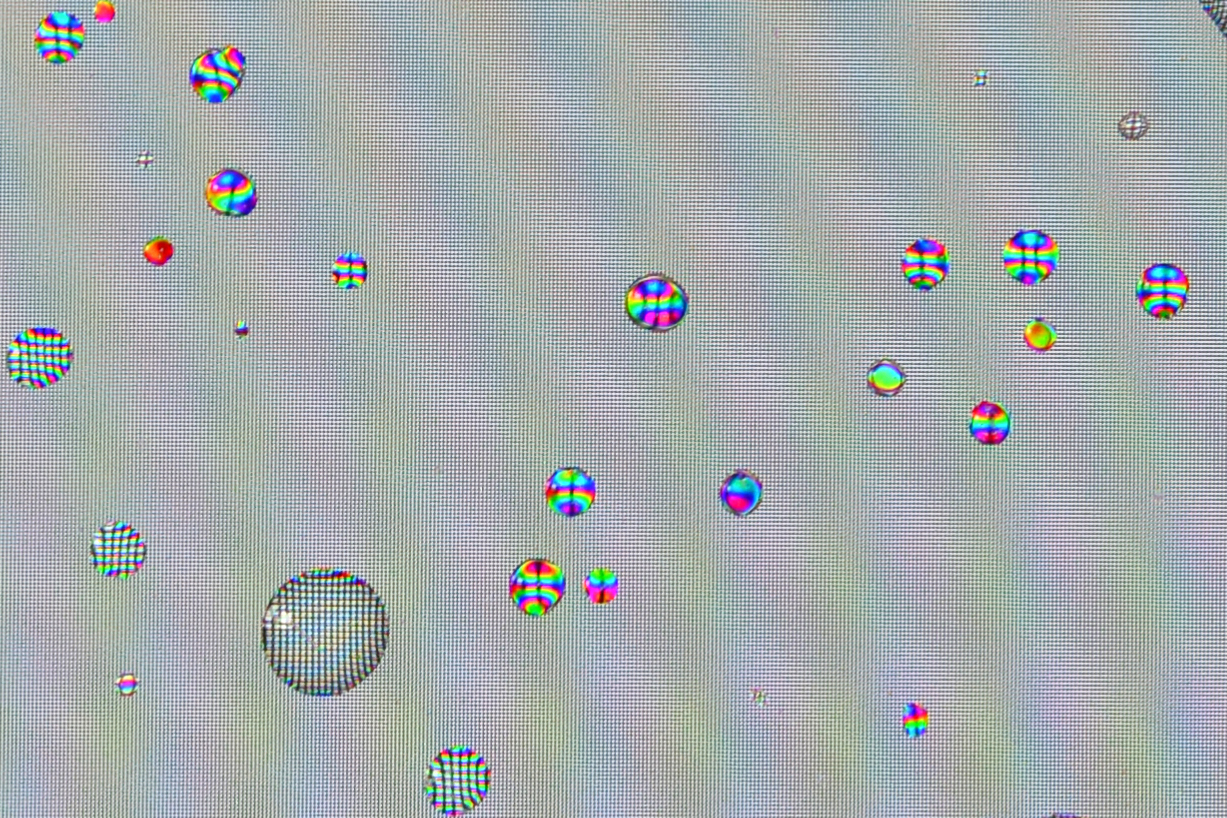
\includegraphics[width=7truecm]{slike/02_photos_kapljice.jpg}
\caption{Drobni tisk na bankovcu vidimo šele z uporabo zbiralne leče (levo). 
Drobne kapljice na zaslonu telefona delujejo kot povečevalna lupa in lahko 
razločimo posamezne rdeče, zelene in modre piksle v prikazovalniku (desno).}
\label{fig:02_photos-1}
\end{figure}

\begin{figure}[!ht]
\centering
\includegraphics[height=7truecm]{slike/02_photos_kozarec.jpg}\hfill
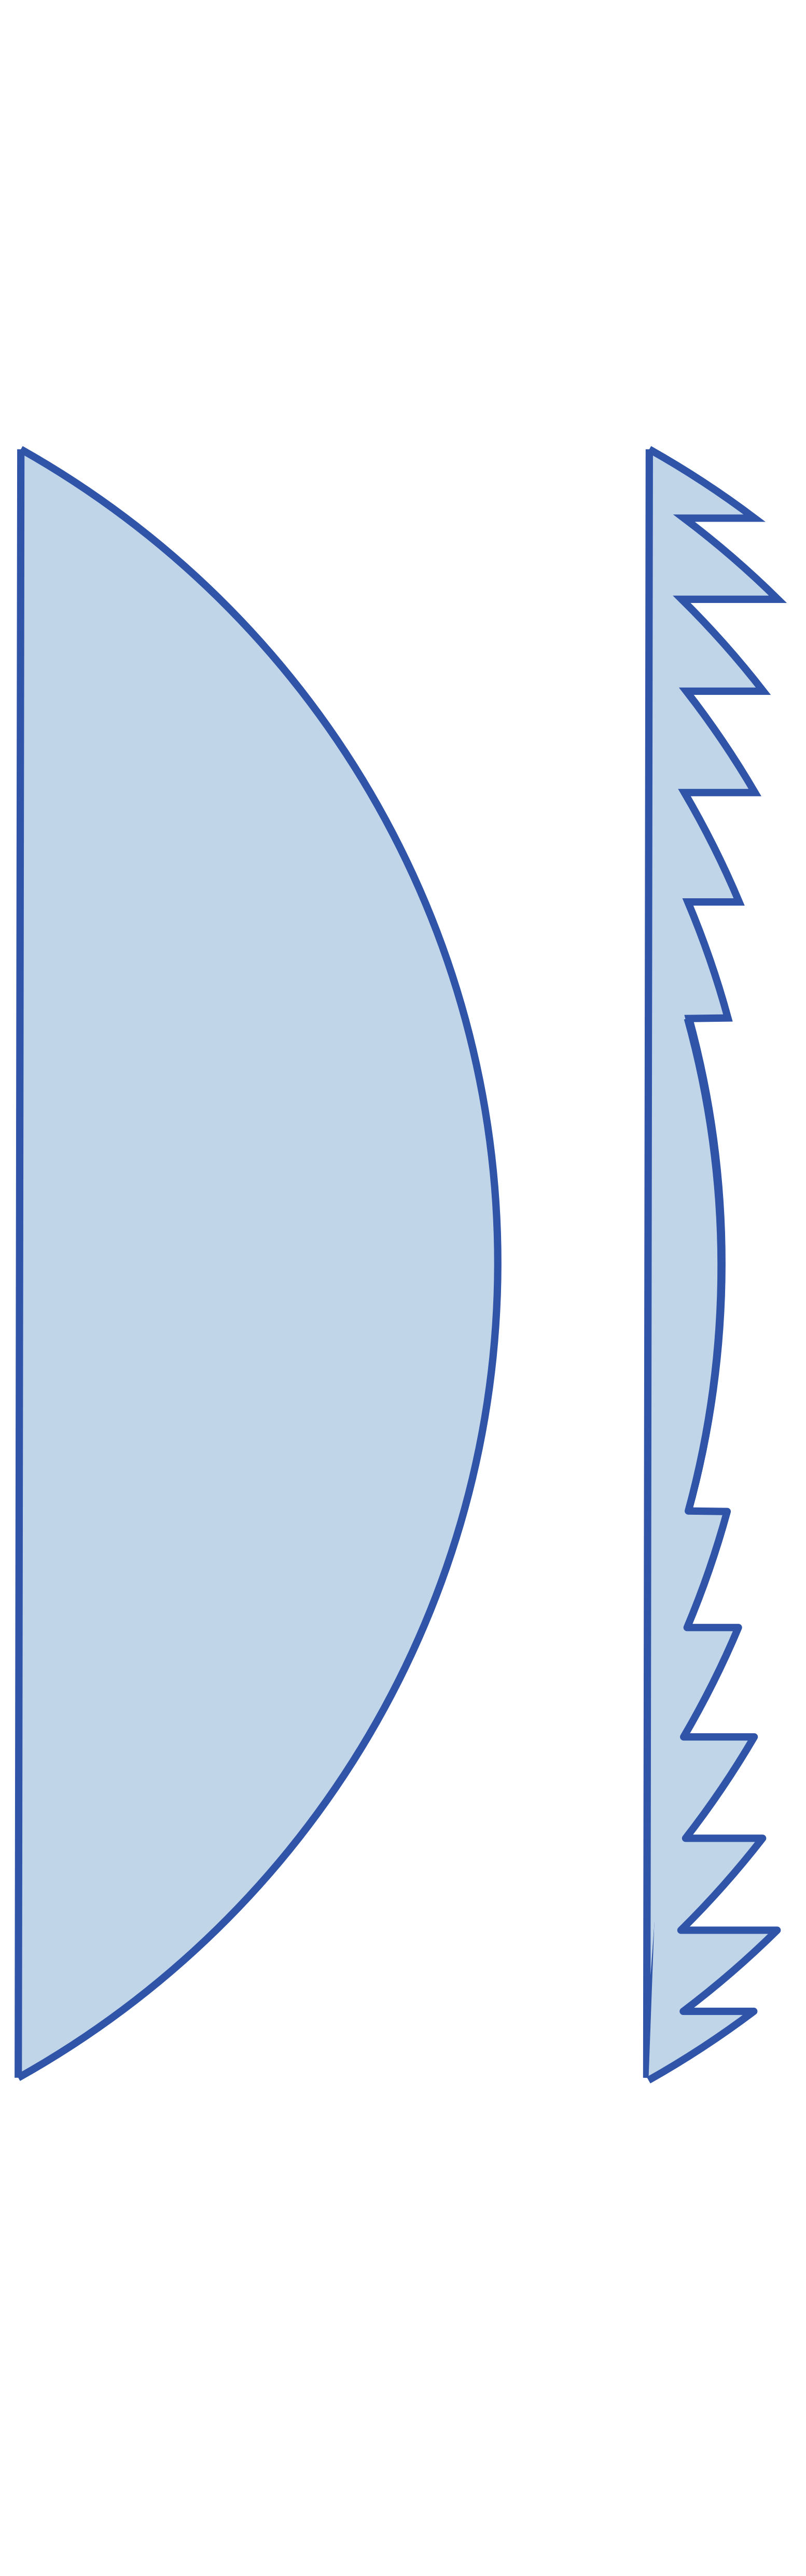
\includegraphics[height=7truecm]{slike/02_FresnelLeca.png}\hfill
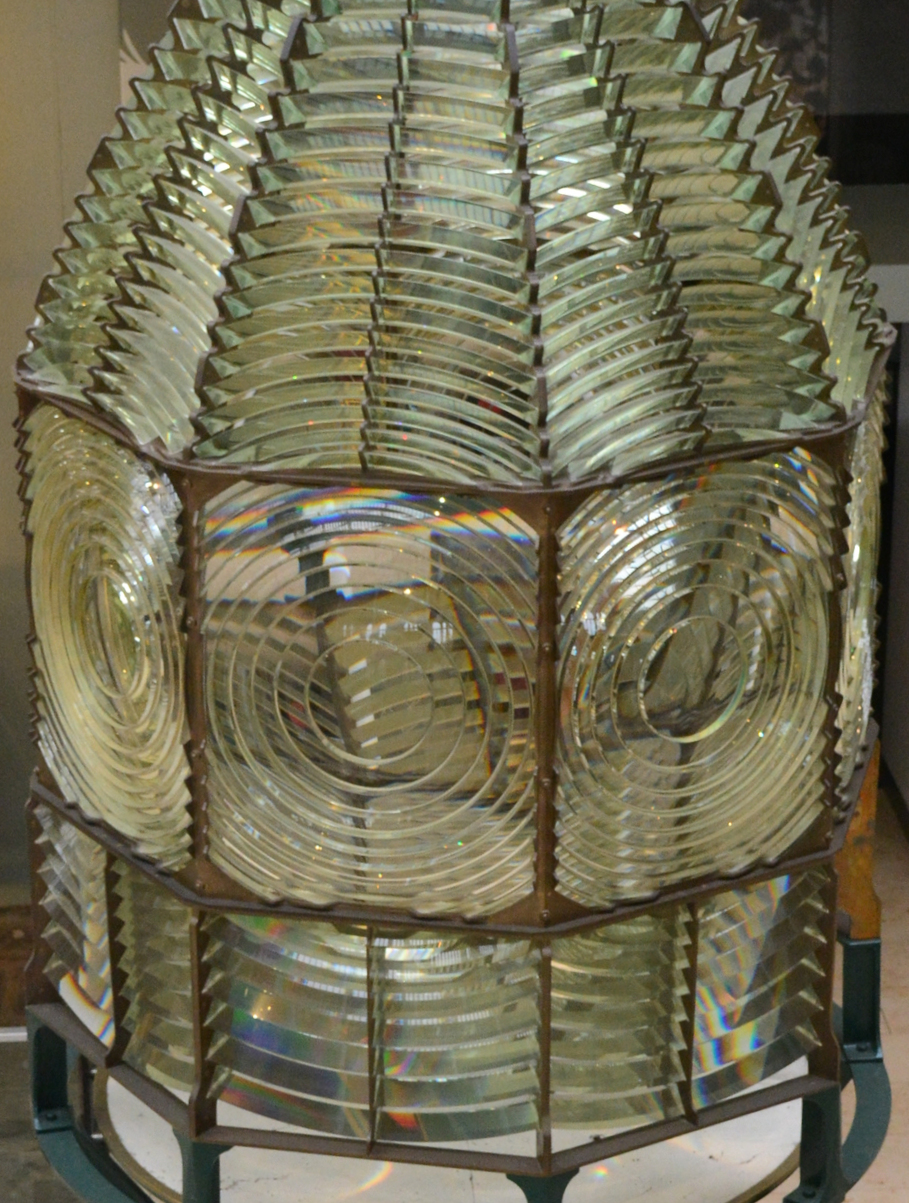
\includegraphics[height=7truecm]{slike/02_photos_svetilnik.jpg}
\caption{Kozarec, napolnjen z vodo, deluje kot zbiralna leča in 
sliko obrne (levo). Shema Fresnelove leče: na posameznih
kolobarjih je enaka ukrivljenost kot na navadni leči, vendar je celotna 
leča tanjša in lažja (sredina). Fresnelova leča na svetilniku ustvari široke 
snope svetlobe, ki so vidni od daleč (desno).}
\label{fig:02_photos-2}
\end{figure}
\vglue-1truecm
\begin{figure}[!ht]
\centering
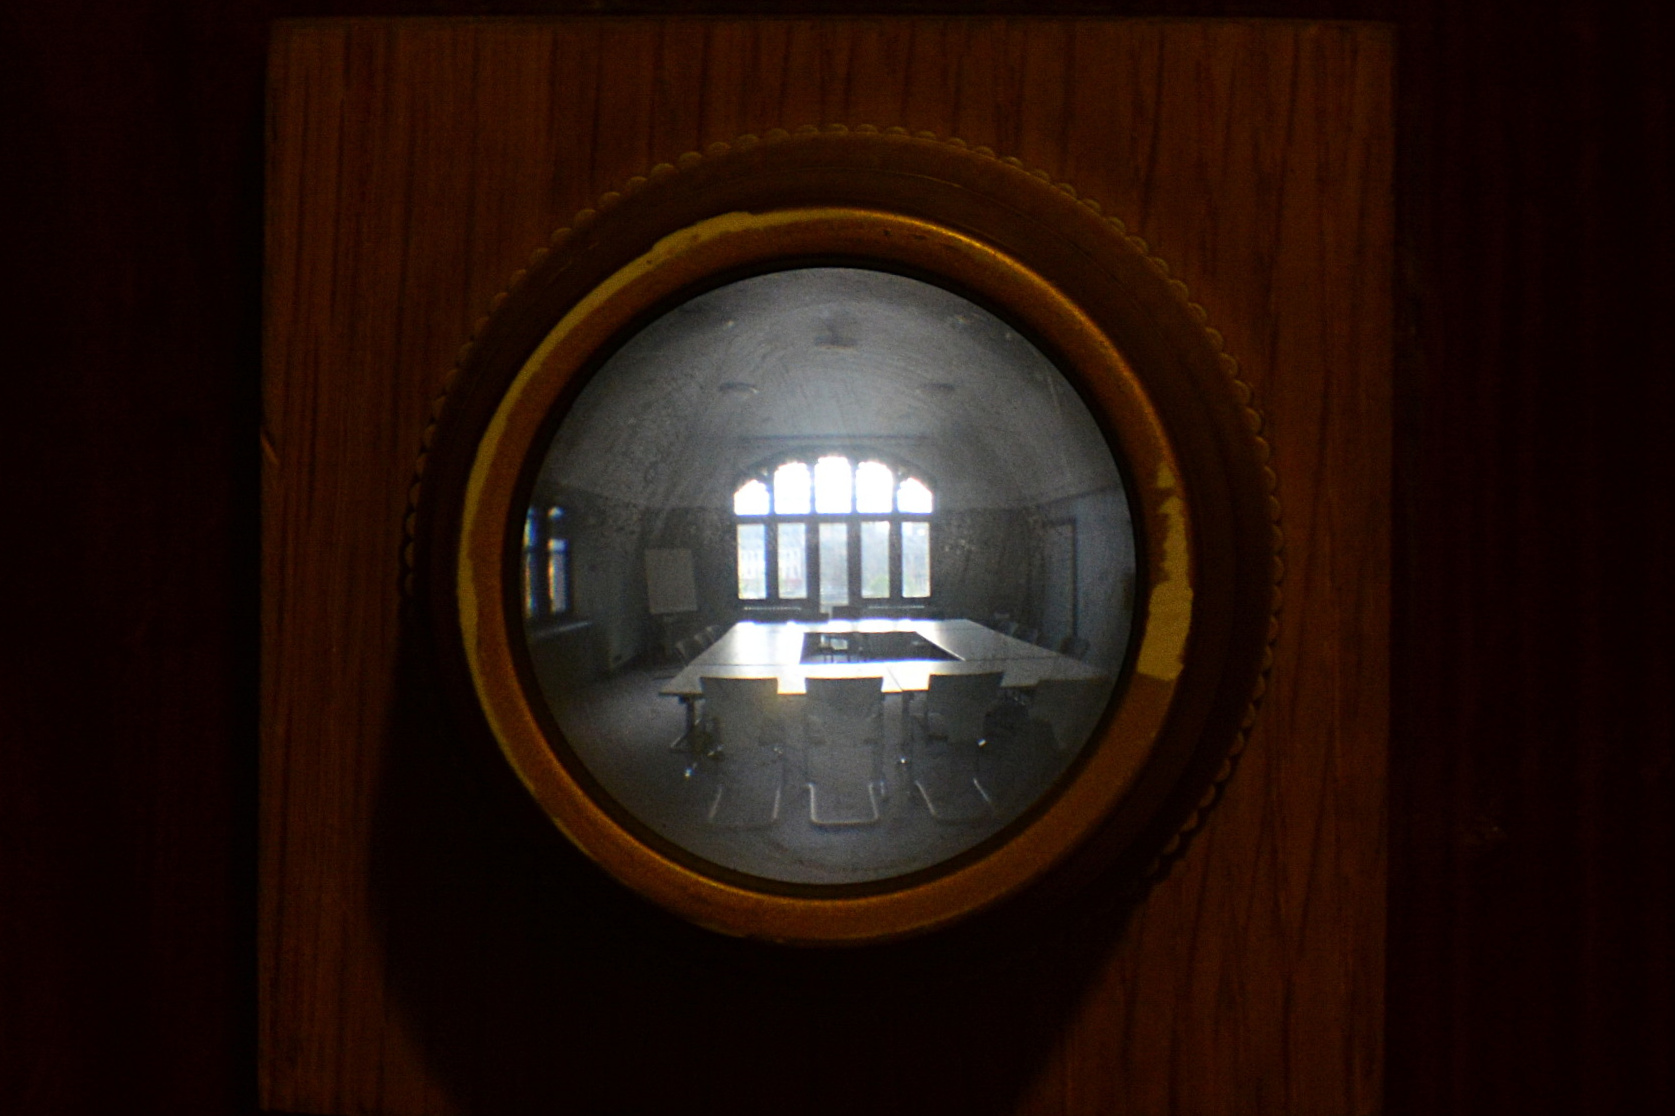
\includegraphics[width=8truecm]{slike/02_photos_peephole.jpg}
\caption{Vratno kukalo uporablja razpršilne leče, da zajamejo čim večjo sliko (levo).}
\label{fig:02_photos-3}
\end{figure}

\newpage
Konveksna zrcala se uporabljajo na primer v avtomobilih kot vzvratna ali v prometu kot
cestna ogledala, da povečamo vidno polje. Podobno delujejo tudi novoletne 
okrasne bunkice ali žlica s hrbtne strani. Konkavna zrcala najdemo v
avtomobilskih žarometih, da zberejo čim več izsevane svetlobe, in za zobozdravniška
ali kozmetična zrcala, da povečajo sliko. Kot konkavno zrcalo deluje tudi 
sprednja stran žlice.

\begin{figure}[!ht]
\centering
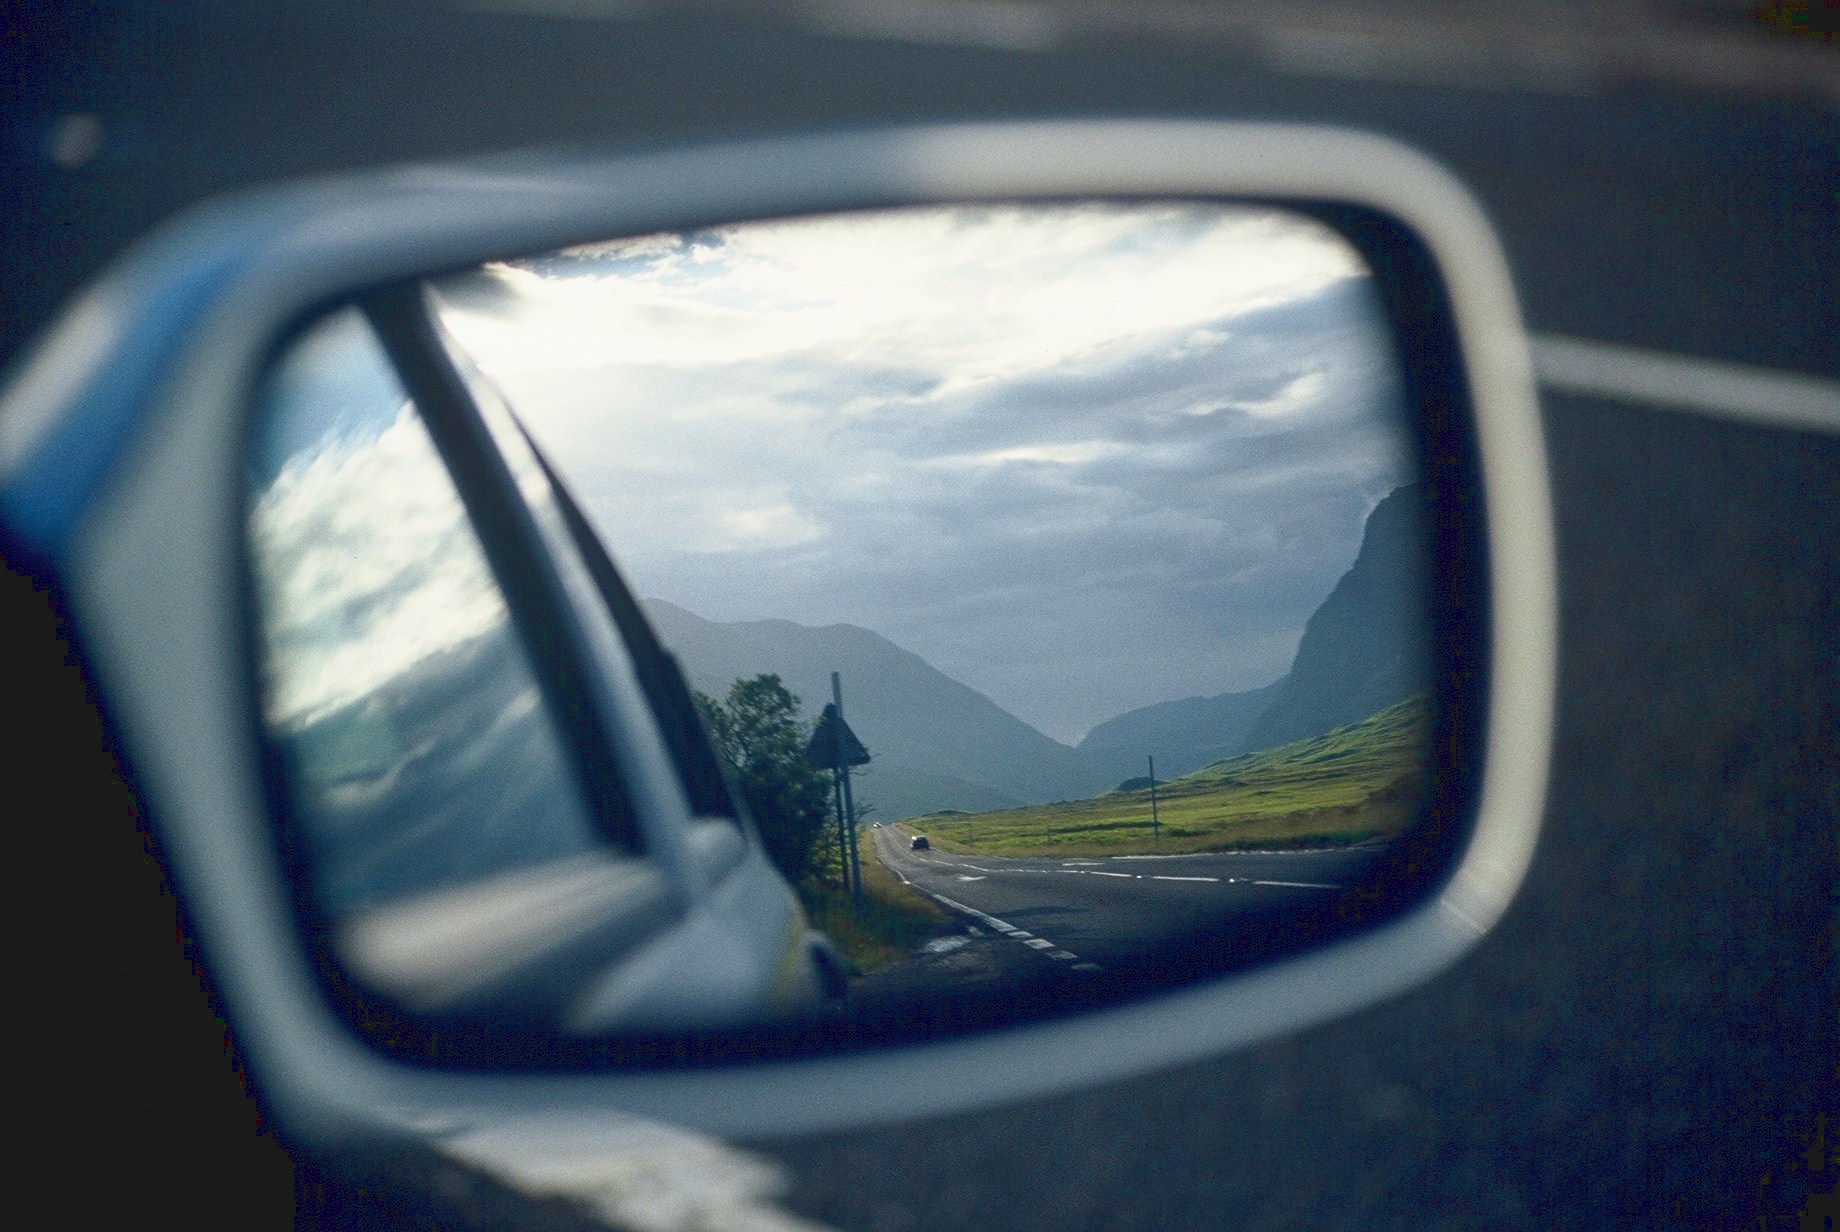
\includegraphics[width=7truecm]{slike/02_photos_avto.jpg}\hfill
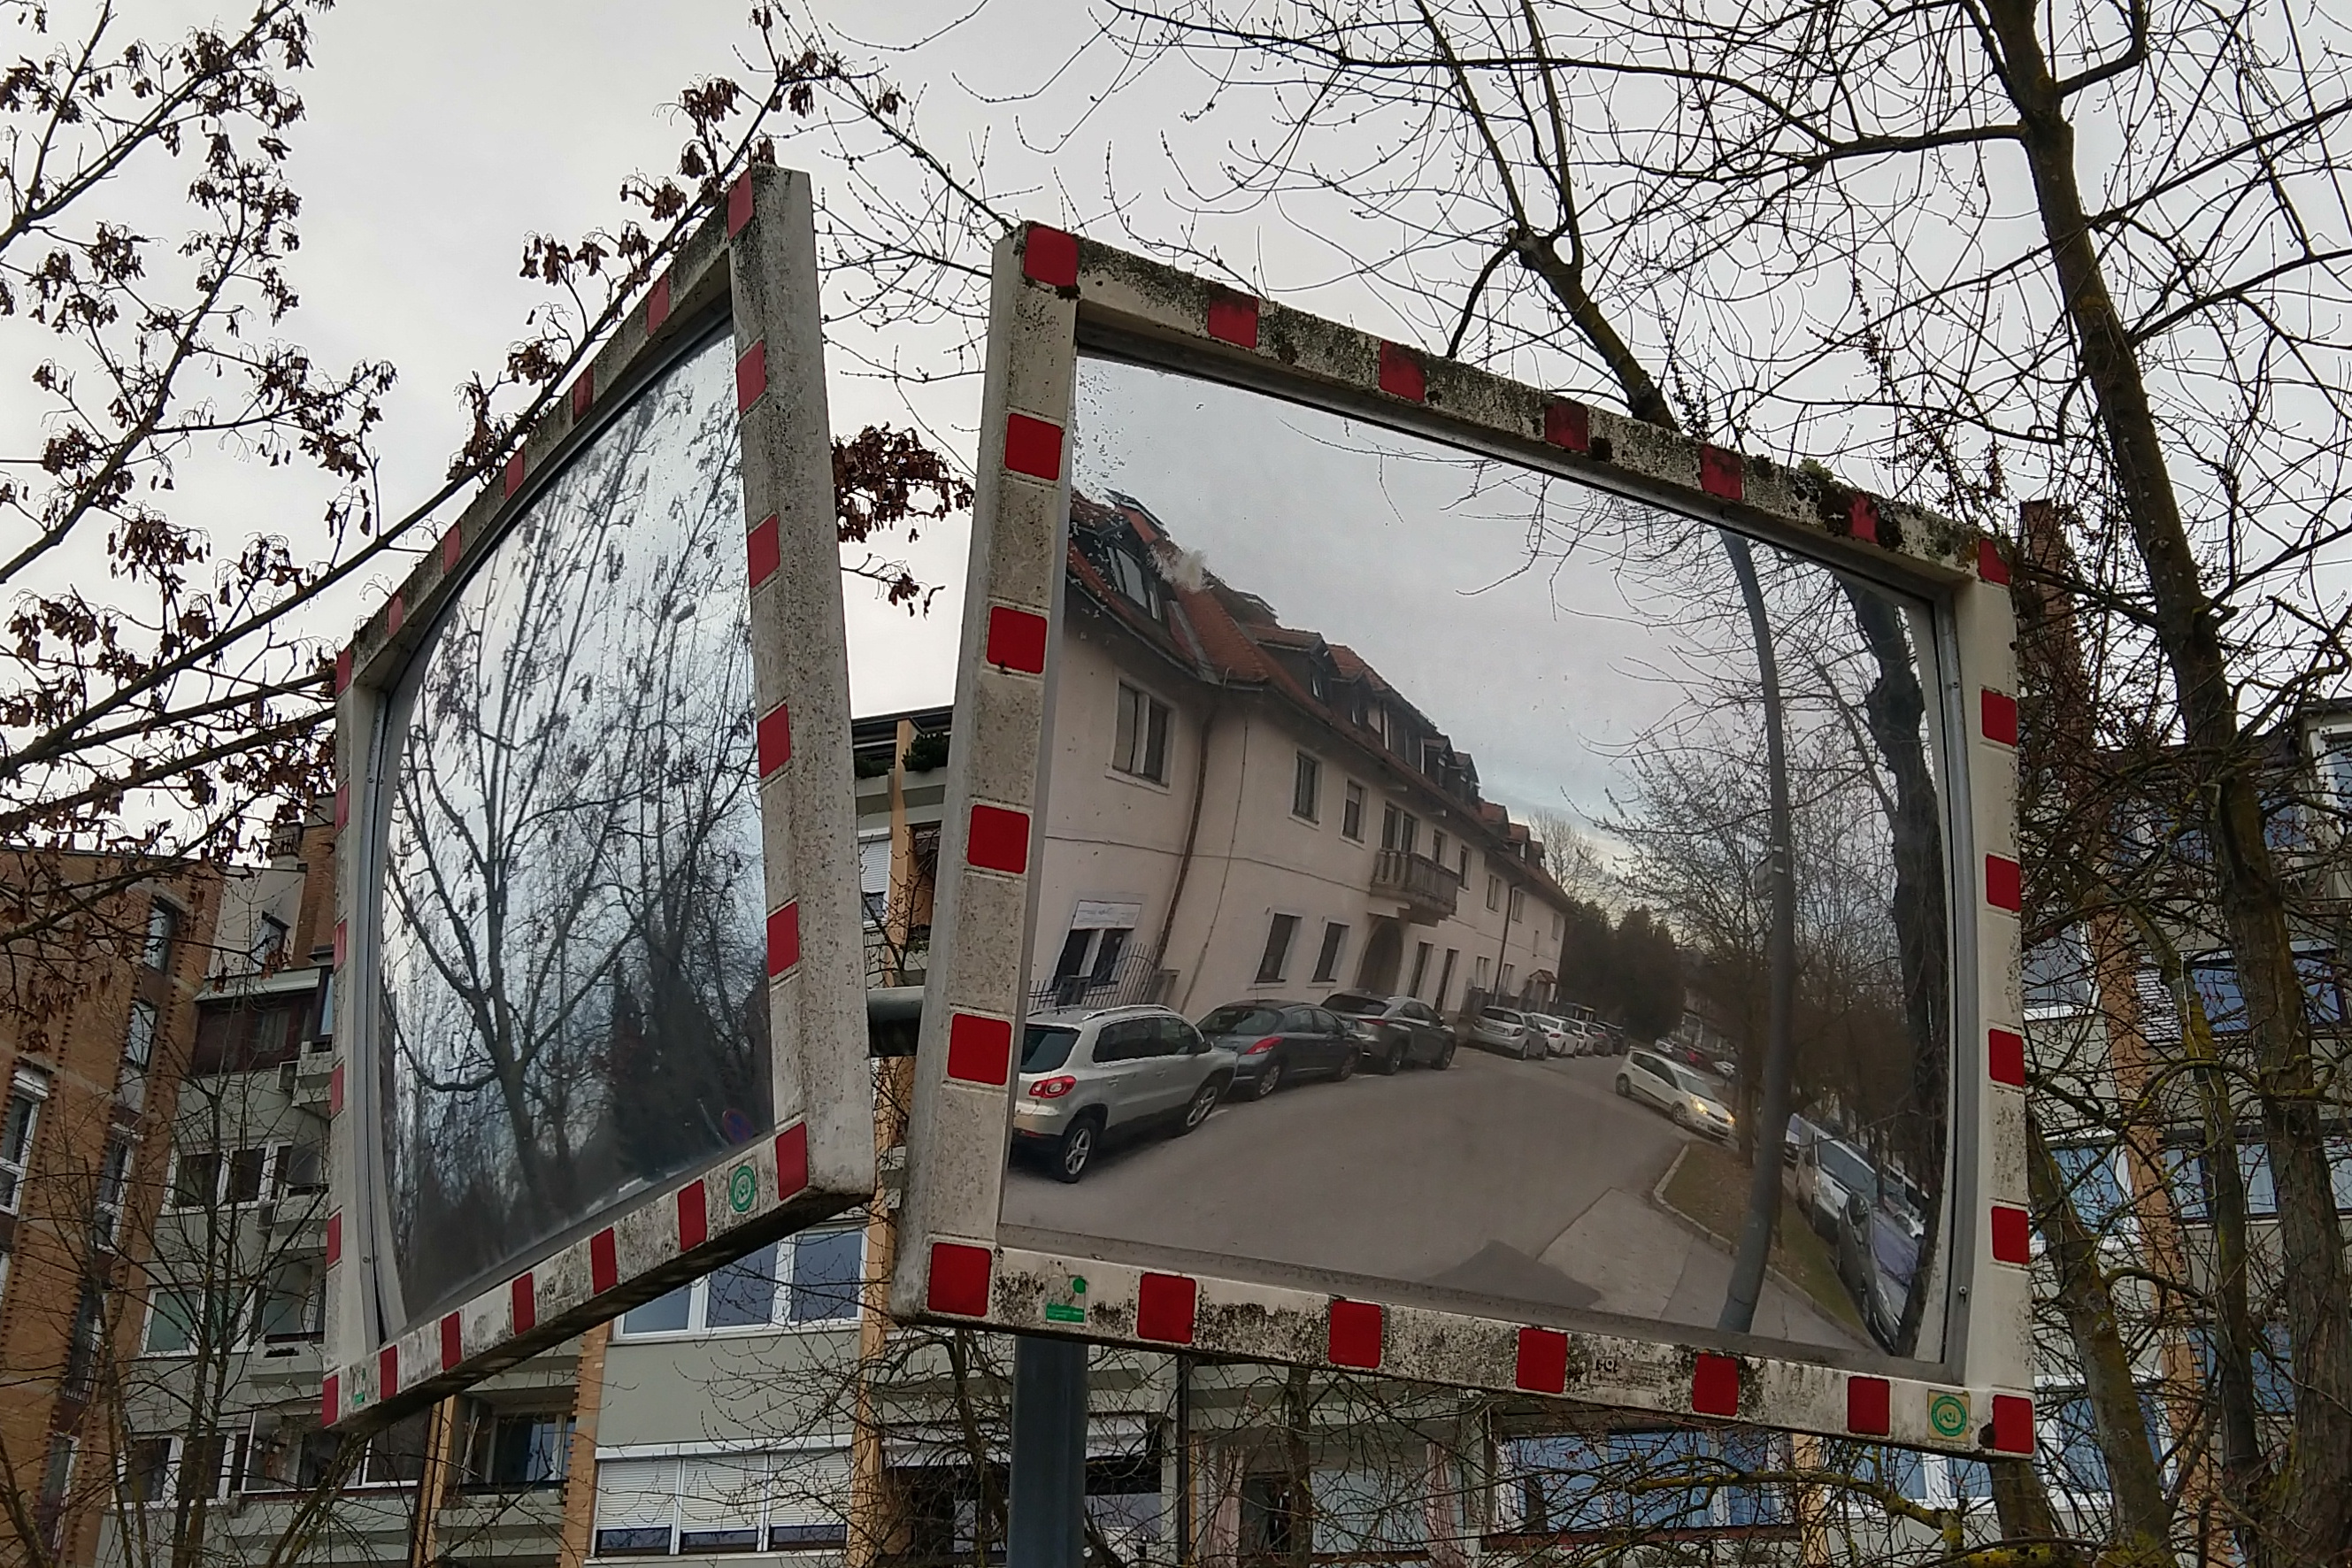
\includegraphics[width=7truecm]{slike/02_photos_cestno.jpg}
\caption{Konveksna zrcala povečajo vidno polje, zato jih uporabljamo v prometu.}
\label{fig:02_photos-4}
\end{figure}

\begin{figure}[!ht]
\centering
\includegraphics[width=7truecm]{slike/02_photos_zlica1.JPG}\hfill
\includegraphics[width=7truecm]{slike/02_photos_zlica2.JPG}
\caption{Žlica lahko deluje kot konveksno (levo) ali konkavno zrcalo (desno).}
\label{fig:02_photos-5}
\end{figure}
